\documentclass[journal]{IEEEtran}
\usepackage[T1]{fontenc}
\usepackage{amsmath}
\interdisplaylinepenalty=2500
\usepackage[cmintegrals]{newtxmath}
\usepackage{booktabs}
\usepackage{array}
\hyphenation{op-tical net-works semi-conduc-tor}
\ifCLASSINFOpdf
\usepackage[pdftex]{graphicx}
\else
\fi
\begin{document}



\title{Software defect prediction based on gated hierarchical LSTMs}

\author{Hao~Wang,
        Weiyuan~Zhuang,
        and~Xiaofang~Zhang% <-this % stops a space
\thanks{H Wang, W Zhuang, and X Zhang are with the School of Computer Science and Technology, Soochow University, Suzhou, 215006, China (e-mail: 20185227067@stu.suda.edu.cn; 20204227007@stu.suda.edu.cn; xfzhang@suda.edu.cn). Corresponding author: Xiaofang~Zhang}}


\markboth{IEEE TRANSACTIONS ON RELIABILITY}%
{Shell \MakeLowercase{\textit{et al.}}: Bare Demo of IEEEtran.cls for IEEE Communications Society Journals}

\maketitle

\begin{abstract}
Software defect prediction, aimed at assisting software practitioners in allocating test resources more efficiently, predicts the potential defective modules in software products. With the development of defect prediction technology, the inability of traditional software features to capture semantic information is exposed, hence related researchers have turned to semantic features to build defect prediction models. However, sometimes traditional features such as lines of code also play an important role in defect prediction. Most of the existing researches only focus on using a single type of feature as the input of the model. In this paper, a defect prediction method based on gated hierarchical Long Short-Term Memory networks (GH-LSTMs) is proposed, which uses hierarchical LSTM networks to extract both semantic features from word embeddings of Abstract Syntax Trees (ASTs) of source code files, and traditional features provided by the PROMISE repository. More importantly, we adopt a gated fusion strategy to combine the outputs of the hierarchical networks properly. Experimental results show that GH-LSTMs outperforms existing methods under both non-effort-aware and effort-aware scenarios.
\end{abstract}


\begin{IEEEkeywords}
software defect prediction, LSTM, hierarchical model, abstract syntax tree
\end{IEEEkeywords}

\IEEEpeerreviewmaketitle

\section{Introduction}

\IEEEPARstart{W}{ith} the scale of software increasing continuously, software defect prediction technology has attracted more and more attention~\cite{catal2009systematic,jiang2013personalized,nam2014survey}. The results given by defect prediction models can help developers or testers to determine whether a software module is defective in the early stage of the software development life cycle so that they can better allocate test resources, arrange the test process more efficiently, and consequently improve the quality of software products.


The traditional software defect prediction models mainly predict whether the program is defective based on the statistics of program characteristics, which assumes that the flawless modules and the defective modules have distinguishing features or feature combinations, such as the total number of lines of code, the number of added or deleted lines of code, the number of changed files, quality features, system complexity features~\cite{maurice1977elements}, Halstead features~\cite{mccabe1976complexity} and so on. By taking these features as inputs of traditional classification algorithms, traditional defect prediction models divide software modules into two categories: buggy or clean, so as to predict defects. However, these approaches ignore the semantic information of the source code, and programs with different semantic features may have similar or even the same traditional features~\cite{wang2018deep}. Under such circumstances, traditional software features are incapable of distinguishing two programs.


In recent years, with the wide application of deep learning, researchers have begun to leverage deep learning to perform effective feature generation for defect prediction. A common practice is utilizing AST parser to extract semantic information from source code files~\cite{wang2018deep}, and then encoding the ASTs into numeric vectors in order to feed them to deep neural networks, which extract semantic features further. But semantic features are not omnipotent and can not represent some information included in traditional features such as the number of lines of code, which is proved rather significant for defect prediction~\cite{zhou2018far}.


%	Because semantic features and traditional features are irreplaceable, some researchers began to concatenate traditional features with semantic features []. The results show that feature fusion can effectively improve the performance of software defect prediction model. However, the existing researches only simply concatenate semantic features with traditional features, which will introduce noise and reduce the performance of the model.


Therefore, we propose a GH-LSTMs model, which extracts both semantic features from word embeddings of ASTs and traditional features provided by the PROMISE\footnote{http://openscience.us/repo/defect} repository using the hierarchical architecture of LSTMs. Additionally, to appropriately determine the combination ratio of the two kinds of features, we introduce the gated fusion mechanism to merge the output of two LSTMs, which utilizes self-learning gates to filter the information passing through.


Our work focuses on with-in project file-level software defect prediction and evaluates prediction performance by means of metrics under both non-effort-aware scenario and effort-aware scenario. Experimental results on 10 projects show that, under non-effort-aware scenario, our proposed GH-LSTMs method outperforms the state-of-the-art methods in terms of $F-measure$. Additionally, under effort-aware scenario, GH-LSTMs achieves better performance than the state-of-the-art methods in terms of $PofB20$ and $IFA$, and comparable performance with the state-of-the-art methods in terms of $P_{opt}$.


The main contributions of this paper are:
\begin{itemize}
	\item We propose a GH-LSTMs model to extract both semantic and traditional software features and effectively combines the extracted features using gated fusion mechanism.
	\item We conduct rigorous experiments to evaluate the performance of the GH-LSTMs model under both non-effort-aware and effort-aware scenarios.
	\item We demonstrate that proper feature fusion can significantly boost the performance of defect prediction.
\end{itemize}


The rest of this paper is summarized as follows: Section 2 introduces the background, including Deep Belief Network (DBN), word embedding, Recurrent Neural Network (RNN), LSTM and the motivation of this paper; A hierarchical gated networks model is introduced in Section 3; Section 4 describes the experimental setup and results, and then demonstrates the potential threats to validity; Section 5 discusses the related work; The conclusion of this paper and the future work are presented in Section 6.

\section{Background}
\subsection{Deep belief network and word embedding in software defect prediction}
%Software defect prediction is a process of predicting code areas that potentially contain defects, which can help developers allocate their testing efforts by first checking potentially buggy code.
Software defect prediction is able to help developers allocate testing resources by predicting potential defects in software modules.
Since software defect prediction is based on the feature extraction of software modules, there are various kinds of software features proposed by existing studies, which can be categorized into two main types: code metrics and process metrics. In recent years, some researchers have proposed semantic features, which are generated by using deep learning technology to extract features from ASTs of source code files automatically. Based on existing studies, semantic features are usually obtained from two techniques: Deep Belief Network~\cite{wang2018deep} and Word Embedding~\cite{fan2019deep,li2017software}.


DBN~\cite{hinton2006fast} is a probability generation model, which establishes a joint distribution between observation results and labels, and performs evaluations in both observation/label direction and label/observation direction. DBN is composed of several Restricted Boltzmann Machines (RBM). Each RBM has two layers of neurons: One layer is called visible layer, which is composed of visible units and used to accept the training data. The other layer is called hidden layer, which consists of hidden units and serves as feature detectors. The training process of an RBM can be described as:
\begin{eqnarray}
P(h_{j}|v)=\sigma(b_{j}+\sum_{(i=1)}^{N}W_{ij}v_{i})
\end{eqnarray}
\begin{eqnarray}
P(v_{i}|h)=\sigma(c_{i}+\sum_{(j=1)}^{M}W_{ij}h_{j})
\end{eqnarray}
Equation (1) is the probability function of the activation result of the neural unit $h_{j}$ in hidden layer, when the state values of all the neurons in visible layer are given. Equation (2) is the probability function of the reconstruction result of a neural unit $v_{i}$ in visible layer, when the state values of all the neurons in hidden layer are given. In these two equations, the common parameter $\sigma$ is the sigmoid function, and $W_{ij}$ is the weight between $i$th neuron in visible layer and $j$th neuron in hidden layer. In addition, $h_{j}$ is the value of $j$th neuron in hidden layer, $v_{i}$ is the value of $i$th neuron in visible layer, $b_{j}$ is the bias of $j$th neuron in hidden layer, $c_{i}$ is the bias of $i$th neuron in visible layer, $N$ is the number of neurons in the visible layer, $M$ is the number of neurons in the hidden layer. The weight and bias matrices are automatically learned through log-likelihood stochastic gradient descent.


DBN is made up of multiple RBMs. To be specific, the hidden layer of the last RBM will be treated as the visible layer of the current RBM. In the training process, each layer of the RBM network is trained independently to ensure that as much feature information as possible is preserved when the feature vectors are mapped to different feature spaces. Then the backpropagation mechanism is set up, where the output vector of an RBM is treated as its input vector to tune the weights between layers in order to make a better reconstruction of the input data before. When all the iterations are finished, a trained DBN model can be obtained to extracted features from the original input data. Semantic software features can be generated according to the process above using the DBN model.

On the other hand, some researchers~\cite{fan2019deep,li2017software} suggest that semantic features can also be generated by word embedding techniques. Compared with DBN, word embedding can make better use of the context of AST node sequences. Normally word embedding is accomplished by word2vec~\cite{mikolov2013distributed} or GloVe (Global Vectors)~\cite{pennington2014glove}.


GloVe is used in this paper to transform an AST node token(as a word) into a vector composed of real numbers, which is calculated based on the semantic relation between words, such as frequency and analogy. First of all, a corpus of the AST node sequences is build and used to construct the co-occurrence matrix. Each element $X_{ij}$ in the matrix represents the number of times that word $i$ and word $j$ appear together in a specific size of the context window. Furthermore, GloVe proposes a decreasing weighting function to calculate the number of co-occurrence: $decay=1/d$, based on the distance $d$ between two words in the context window, to calculate the weight, i.e., the longer the distance, the less the weight of two words in the total count. After the co-occurrence matrix is built, the GloVe model can be trained based on this loss function:
\begin{equation}
J=\sum_{i,j=1}^{V}f(X_{ij})(\omega_{i}^{T} \tilde{\omega}_{j}+b_{i}+\tilde{b}_{j}-\log(X_{ij}))^{2}
\end{equation}
where $V$ is the size of the vocabulary, $\omega_{i}$ and $\tilde{\omega}_{j}$are the expected word vectors, $b_{i}$ and $\tilde{b}_{j}$ are the bias term of the two word vectors respectively, $f(X_{ij})$ is the weighting function, which is defined as follows:
\begin{equation}
f(x)=
\begin{cases}
(x/x_{max})^{\alpha}\quad \ \ & if\ x<x_{max}\\
1\quad \ \ & oterwise
\end{cases}
\end{equation}
where $\alpha$ and $x_{max}$ are adjustable parameters of the weighting function.

Semantic software features presented in the form of word embedding can be obtained according to the process above using GloVe.

\subsection{Recurrent Neural Network in software defect prediction}
%Recurrent Neural Network(RNN) performs well in sequential tasks such as Natural Language Processing tasks where inputs data might have a sequential relationship. The main point of RNN is that it can save internal state (memory) to process sequences of inputs. Nodes in RNN are organized into successive hidden layers, and each hidden layer not only has an output value, but also has a state value (memory) that can be influenced by both the input value of this layer and the state value of last layer. LSTM~\cite{hochreiter1997long} is an improved variant of basic RNN. A typical LSTM cell is shown in Fig.~\ref{fig2}. LSTM employs three gates, input gate, forget gate and output gate to avoid vanishing gradient and exploding gradient that tends to show up during the training of basic RNN. The forget gate is used to determine how much of the state value of last layer should be added to the state value of this layer; the input gate is used to determine how much of the input value of this layer should be added to the state value of this layer, and the output gate is used to determine how much of the state value of this layer should be added to the output of this layer. Each gate has its own weight matrix and bias term, which can be learned during the training process.

Recurrent Neural Network(RNN) achieves outstanding performance in processing sequential data with the help of its inner recurrent architecture. RNN processes the input sequence by traversing all elements and saving a state memory that contains information about what has been viewed. LSTM~\cite{hochreiter1997long}, as an improved variant of basic RNN, is designed to solve the problem of vanishing gradient and exploding gradient during the training of traditional RNN. A typical LSTM cell is shown in Fig.~\ref{fig2}. LSTM makes use of three gates to control the input and output streams of information. The forget gate determines how much of the state memory from last time step will be reserved to the current time step; the input gate determines how much of the current input will be saved to the current state memory; and the output gate is used to control how much of the current state memory should be output in the current time step. There are a weight matrix and a bias term for each gate, which will be automatically learned in the training phase.


With the development of software defect prediction technology, many studies~\cite{fan2019deep,liang2019seml,liu2018connecting} use RNN to establish classifiers and perform feature extraction with the purpose of achieving better prediction results.
\begin{figure}[htbp]
	\centering
	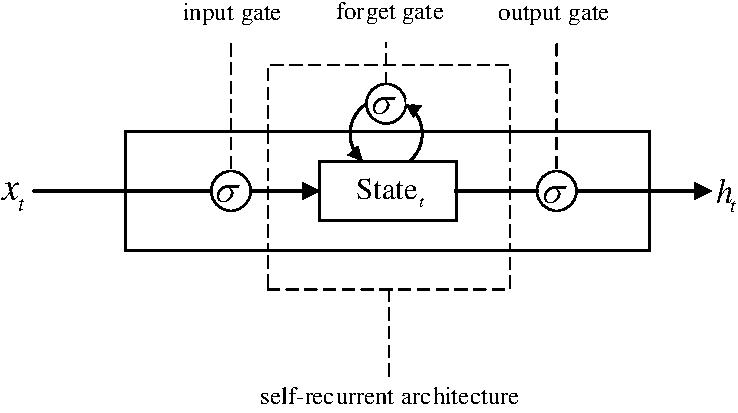
\includegraphics[scale=0.65]{figs/LSTM_model.pdf}
	\caption{LSTM model}
	\label{fig2}
\end{figure}

\subsection{Motivation}
Based on previous studies, there are two types of software defect prediction features: traditional features and semantic features. On the one hand, semantic features can capture the semantic information of code snippets that traditional features are unable to represent. For example, there are two Java files in Fig.~\ref{fig1}, file 1(clean) and file 2(buggy) have the same code statements only with different positions of the statement `start=1;'. If we use traditional features such as code complexity features to describe these two code snippets, we will get the identical results, thus unable to distinguish the buggy file. On the other hand, only using semantic features will also lose some statistical information about source code, such as the LOC feature, which is significant for defect prediction~\cite{zhou2018far} but can not be obtained from semantic features. To sum up, traditional features are shown to be informative in distinguishing buggy code while semantic features perform better in capturing semantic information of code. This encourages us to design a defect prediction method that makes use of both kinds of features.
\begin{figure*}[htbp]
	\centering
	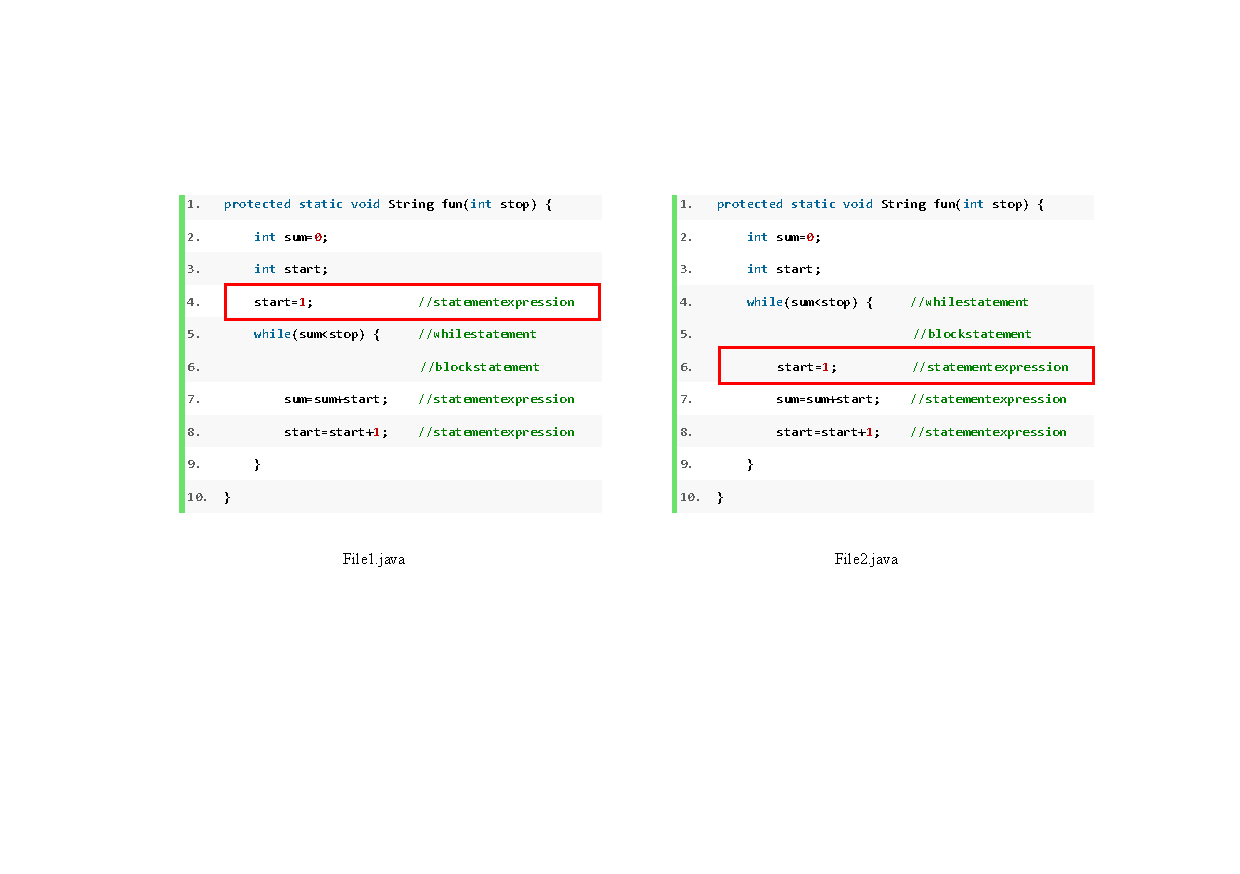
\includegraphics{figs/example.pdf}
	\caption{A concrete example}
	\label{fig1}
\end{figure*}

The challenge to proper feature combination is how to determine the reasonable ratios of two kinds of features since the performance of each feature in defect prediction may vary in different software. To solve this problem, we propose a novel model named Gated Hierarchical LSTMs. It leverages a powerful hierarchical LSTMs architecture to ensure the full extraction of each feature and utilizes a self-learning gated fusion mechanism to automatically determine the optimal ratio in feature combination.


\section{Approach}
\label{approach}

Most of the existing studies only focus on one kind of feature, or simply do concatenation of different features. In order to make the best use of both kinds of features, inspired by our previous work~\cite{wang2018gated}, we designed a gated hierarchical LSTMs model for defect prediction, which is capable of taking full advantage of both semantic features and traditional features. Fig.~\ref{fig3} shows the whole framework of our method.
\begin{figure*}[!h]
	\centering
	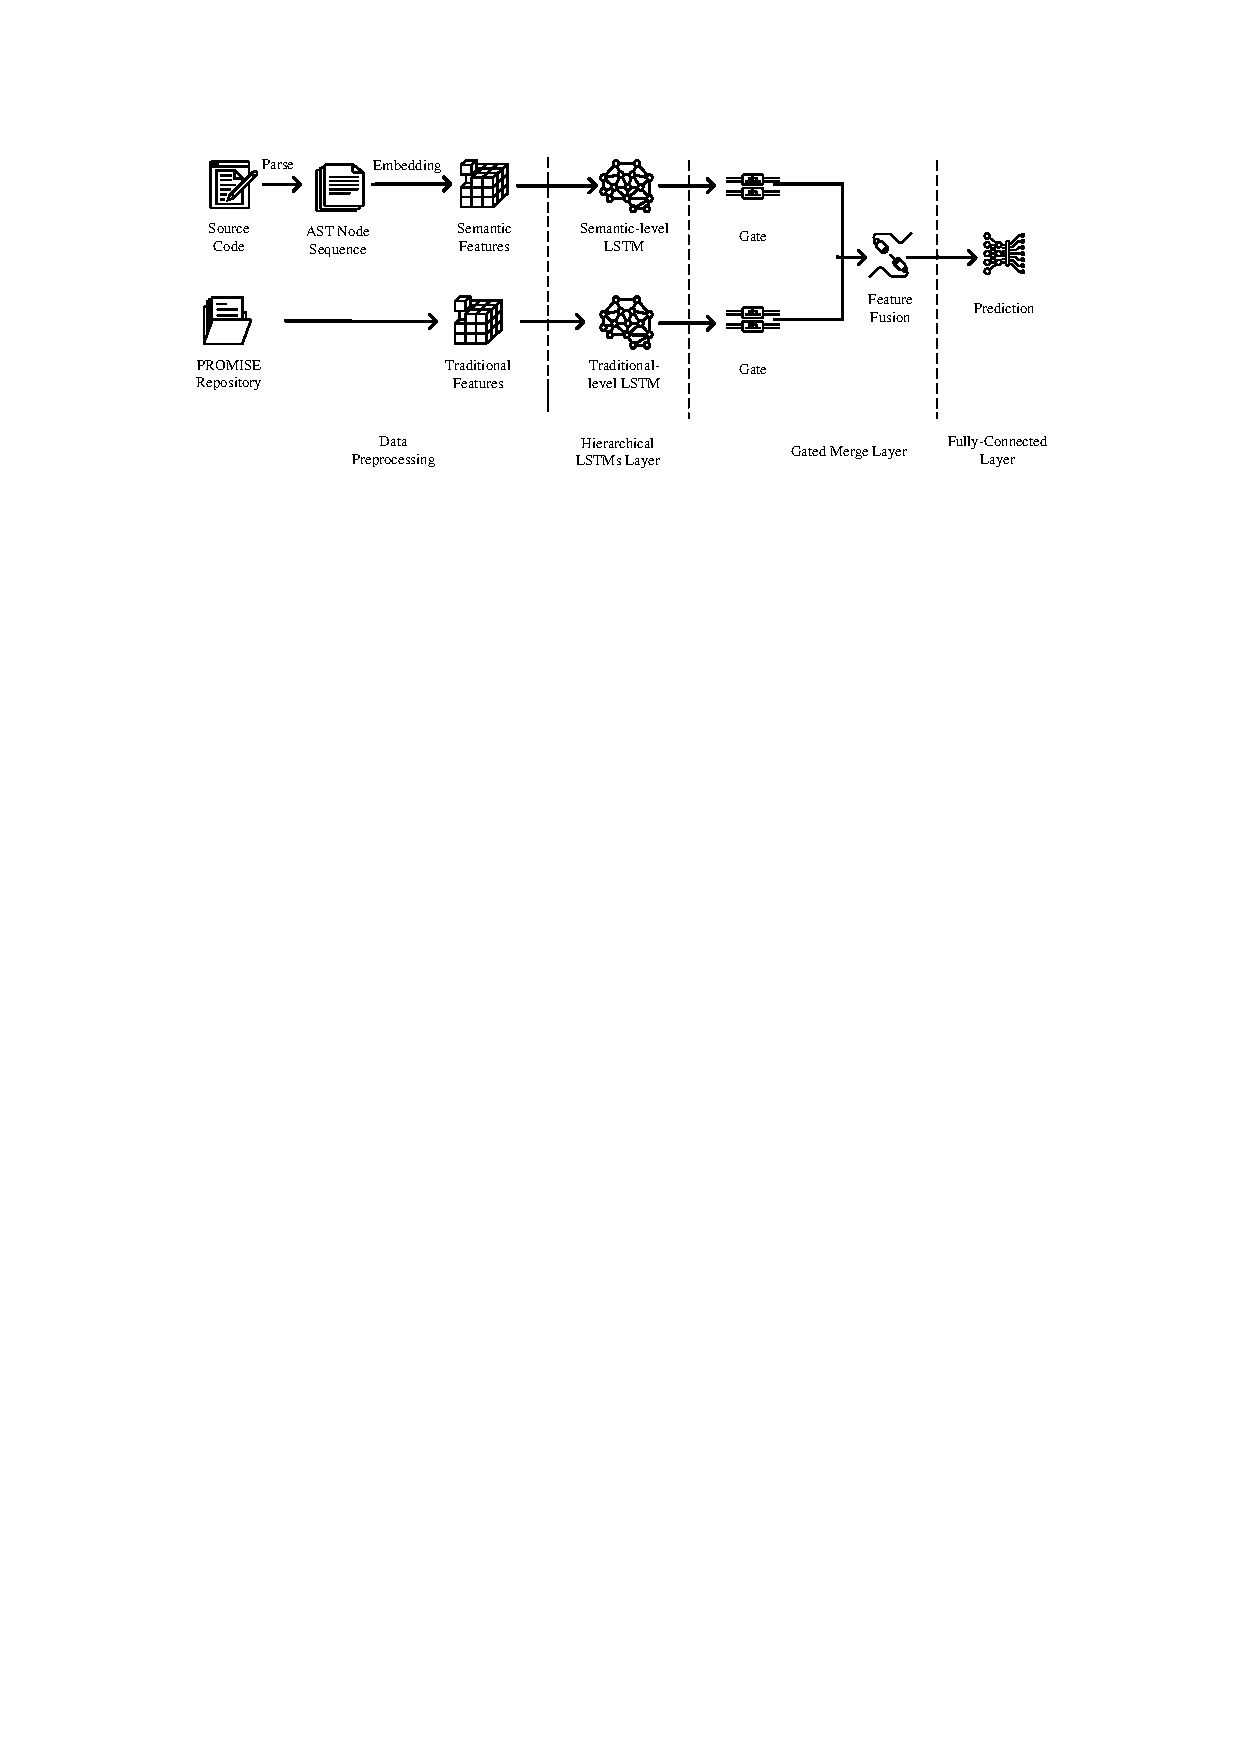
\includegraphics[scale=1.10]{figs/GH-LSTMs.pdf}
	\caption{GH-LSTMs}
	\label{fig3}
\end{figure*}
%First, we search the source code files of each project and their traditional features, then extract the AST nodes from the source code file, and initialize all the extracted AST node sequences by GloVe as corpus. In addition, we use corpus to map AST nodes to multi-dimensional vectors as semantic features. Then, we put semantic features and traditional features into two identical LSTMs to further learn the effective information. Furthermore, considering that the feature information may have noises, we put the output of LSTMs into the gated layers to filter the noise and concatenate the output of the two gated layers. Finally, we use the combined digital vector to predict whether each file is faulty or non-faulty.

First, we manage to extract semantic features and traditional features during data preprocessing. Then the two kinds of features will be taken as inputs to a hierarchical LSTMs to make a further extraction of the hidden information of each feature. After that, the outputs of hierarchical LSTMs will be fed into a gated merge layer where feature fusion happens under the control of gated mechanism. Finally, we input the combined feature into a fully-connected layer to get the defect distribution, i.e., clean or buggy.

\subsection{Data preprocessing}
\label{data_preprocessing}
To extract the semantic feature of source code files, we firstly parse source files into AST token sequences, which reserves the semantic information of code. For each source code file, an AST token sequence is generated. Then we join the sequences from the same project together to produce a semantic code corpus, which will be used by GloVe to train the word embedding model for this project. Once the word embedding model is acquired, it can be used to generate the vector representation of AST token sequence, i.e., the semantic feature that used in our work.

For traditional features, we selected 18 code metrics provided by the PROMISE repository according to previous studies~\cite{wang2018deep,fan2019deep,ni2019empirical}.

\subsection{Hierarchical LSTMs}
In order to utilize both semantic features and traditional features, we construct a hierarchical LSTMs model composed of a semantic-level LSTM and a traditional-level LSTM. As Fig.~\ref{fig3} shows, the input of the semantic-level LSTM is a sequence made up of semantic word vectors. Each LSTM unit receives the output vector from the last LSTM unit and input vector of the current time step, which is defined as
\begin{equation}
E_{s}=W_{h}\cdot h_{(i-1)} \oplus W_{x}\cdot x_{i}
\end{equation}
In which $h_{(i-1)}$ refers to the output of previous hidden layer, $W_{h}$ refers to the weight matrix of the hidden layer, $x_{i}$ refers to the $i$th input vector, $W_{x}$ refers to the weight matrix of the input vector, and $\oplus$ refers to the concatenation operation. With the iteration of $i$ continuing, the extracted information will be added into $E_{s}$ sequentially.

Similarly, for traditional features, we treat the 18 code metrics as a sequence containing 18 time-steps and feed the sequences into the traditional-level LSTM to extract hidden information in the same way as semantic-level LSTM.

\subsection{Gated merge layer}
The highlight of our method is that we figure out a proper way to automatically determine the best proportion of each kind of feature during the fusion phase. We feed the outputs of semantic-level LSTM and traditional-level LSTM into a gate function separately, where a fully-connected layer is used to generate a filter for the information passing through. Then the gated results will be merged by simple concatenation to generate the combined feature, defined as
\begin{equation}
H_{m}=concatenate(h_{t} \otimes \sigma(W_{t} \cdot h_{t} + b_{t} ), h_{s} \otimes \sigma(W_{s} \cdot h_{s} + b_{s}))
\end{equation}
where $h_{t}$ represents the final output of the traditional-level LSTM, $h_{s}$ represents the final output of the semantic-level LSTM, $W_{t}$, $b_{t}$, $W_{s}$ and $b_{s}$ are learned parameters of the gates, $\sigma$ is the sigmoid function, $\otimes$ is element-wise product, and $concatenate$ represents simple concatenation function.

\subsection{Model training}
%Finally, the output $H_{m}$ of gated merge layer is fed into a softmax layer to predict whether the file is defective or not:
In this step, a softmax layer is used to receive the output $H_{m}$ of gated merge layer and predict whether the file is defective or not:
\begin{equation}
y=softmax(W \cdot H_{m} + b)
\end{equation}
%where $W$ and $b$ are the parameters for the softmax layer.
In which $W$ is the weight matrix of the softmax layer, and $b$ is the bias item.


%We use the backpropagation algorithm to train the model and optimize the model by minimizing the cross-entropy error of defect classification:
The backpropagation algorithm is used during model training, trying to minimize the cross-entropy error of defect classification to optimize the model:
\begin{equation}
loss=-\sum_{(i\in D)}\sum_{(j\in C)}\hat{y}_{i}^{j}\log y_{i}^{j}+\lambda||\theta||^{2}
\end{equation}
where $D$ represents all training instances, $C$ is the result categories (buggy or clean), $\hat{y}$ refers to the correct distribution of results, $y$ is the predicted distribution of result, and $\lambda||\theta||^{2}$ represents $l_2$ regularization.


\section{Experiments settings}
\subsection{Evaluated projects and datasets}
It is necessary to get the correct defect labels of the source code files to build training/testing datasets. We choose to use publicly available data from the PROMISE~\cite{he2013learning} repository, which is a widely used repository in defect prediction studies~\cite{wang2018deep,fan2019deep,li2017software,he2013learning,jing2014dictionary,chen2020different}. Specifically, based on these previous studies, we selected 10 open-source java projects from PRMOISE repository for the convenience of estimating the performance of our proposed method. PROMISE datasets provide file names, defect labels, and traditional code metrics for different versions of various software projects. According to the projects and version numbers in the repository, we locate the corresponding source code files from GitHub\footnote{https://github.com/} and Apache\footnote{https://www.apache.org/} official websites. Table~\ref{tab1} shows the basic information of all the projects we used, including version numbers, the average number of files, and the average bug rate of each project. The average number of source code files of all projects is 414, and the average bug rate of all projects is 29.5\%.

\begin{table}[htbp]
	\footnotesize
	\caption{Dataset description}
	\label{tab1}
	\tabcolsep 11pt
	\centering
	\begin{tabular}{llll}
		\toprule
		Project & Versions & Avg files & Avg bug rate (\%) \\\midrule
		ant     & 1.5, 1.6, 1.7 & 463    & 19.8\\
		camel   & 1.2, 1.4, 1.6 & 815    & 23.9\\
		jedit   & 3.2, 4.0, 4.1 & 296.7  & 27.6\\
		log4j   & 1.0, 1.1      & 122    & 29.6\\
		lucene  & 2.0, 2.2, 2.4 & 260.7  & 54.9\\
		xalan   & 2.4, 2.5      & 763    & 31.7\\
		xerces  & 1.2, 1.3      & 446.5  & 15.7\\
		ivy     & 1.4, 2.0      & 399    & 6.7 \\
		synapse & 1.0, 1.1, 1.2 & 220.3  & 22.6\\
		poi     & 1.5, 2.5, 3.0 & 354.7  & 62.5\\
		Avg     & -             & 414.9  & 29.5\\
		\bottomrule
	\end{tabular}
\end{table}
The semantic features are learned from the AST token sequences of the source code files. We use \textit{javalang}, an open-source Python library, to extract AST token sequences from the source code files. According to existing study[6], we only extracted three categories of AST nodes: method invocation type, declaration type and control-flow type with the intention of avoiding the noise that might be introduced by some specific AST node types such as intrinsic type declaration. The details of selected AST nodes are presented in Table~\ref{tab2}. Then the extracted AST token sequences will be used to build semantic code corpus for training a GloVe model as described in Section~\ref{data_preprocessing}, which later will be used to generate semantic features. As for the traditional feature, we selected 18 code metrics provided by the PROMISE repository like the existing researches~\cite{wang2018deep,fan2019deep} and use them as the traditional feature inputs for our GH-LSTMs model, the details of these code metrics are presented in Table~\ref{tab3}.

\begin{table}[htbp]
	\footnotesize
	\caption{The selected AST nodes}
	\label{tab2}
	\tabcolsep 22pt
	\centering
	\begin{tabular}{ll}
		\toprule
		ReferenceType        & MethodInvocation \\
		MethodDeclaration    & TypeDeclaration\\
		ClassDeclaration     & EnumDeclaration\\
		IfStatement          & WhileStatement        \\
		DoStatement          & ForStatement          \\
		AssertStatement      & BreakStatement        \\
		ContinueStatement    & ReturnStatement       \\
		ThrowStatement       & SynchronizedStatement \\
		TryStatement         & SwitchStatement       \\
		BlockStatement       & StatementExpression   \\
		TryResource          & CatchClause           \\
		CatchClauseParameter & catchclauseparameter  \\
		switchstatementcase  & forcontrol            \\
		enhancedforcontrol   &                \\
		\bottomrule
	\end{tabular}
\end{table}


\begin{table*}[htbp]
	\footnotesize
	\caption{Traditional features selected from PROMISE datasets}
	\label{tab3}
	\tabcolsep 50pt
	\centering
	\begin{tabular}{ll}
		\toprule
		Measure of Functional Abstraction (MFA) & Inheritance Coupling (IC)             \\
		Coupling Between Methods (CBM)          & Response for a Class (RFC)            \\
		Data Access Metric (DAM)                & Efferent couplings (Ce)               \\
		Coupling between object classes (CBO)   & Measure of Aggregation (MOA)          \\
		Lines of Code (LOC)                     & Weighted methods per class (WMC)      \\
		Afferent couplings (Ca)                 & Depth of Inheritance Tree (DIT)       \\
		Number of Children (NOC)                & Lack of cohesion in methods (LCOM3)   \\
		Lack of cohesion in methods (LCOM)      & Cohesion Among Methods of Class (CAM) \\
		Average Method Complexity (AMC)         & Number of Public Methods (NPM)\\
		\bottomrule
	\end{tabular}
\end{table*}

\subsection{Baseline setting}
In this paper, we select the following three baseline methods as comparative methods to estimate the performance of our proposed GH-LSTMs:
\begin{itemize}
	\item DBN~\cite{wang2018deep}(DBN Feature + LSTM): LSTM model with semantic features generated by DBN.
	\item SCE~\cite{liang2019seml}(Semantic-Code-Embedding + LSTM): LSTM model with semantic features generated by word embedding.
	\item DP-AM~\cite{fan2019deep}: A single bidirectional recurrent neural network based on attention mechanism with semantic features generated by word embedding and auxiliary input of traditional features provided by PROMISE repository. Note that DP-AM does not leverage a hierarchical architecture of networks, which means that the traditional features are combined with the extracted semantic information by simple concatenation.
\end{itemize}


For each project listed in Table~\ref{tab1}, we choose every two consecutive versions to build the training and testing datasets to evaluate the performance of a defect prediction method. Specifically, we use the earlier version of two versions to build the training set to train the defect prediction model, and then use the later version to build the testing set for evaluation. In total, we conduct 16 sets of experiments on 10 projects for every method.
\subsection{Evaluation}
\subsubsection{Metrics for non-effort-aware evaluation}
In non-effort-aware evaluation, we choose $F-measure$~\cite{jiang2008techniques} as the evaluation metric, which is widely used in software defect prediction~\cite{wang2018deep,fan2019deep,jing2014dictionary,menzies2006data}. $F-measure$ is defined as the harmonic mean of $Precision$ and $Recall$. The detailed definitions are shown as follows:
\begin{equation}
Precision=\frac{True\;Positive}{True\;Positive + False\;Positive}
\end{equation}
\begin{equation}
Recall=\frac{True\;Positive}{True\;Positive + False\;Negative}
\end{equation}
\begin{equation}
F-measure=\frac{2*P*R}{P+R}
\end{equation}
In defect prediction tasks, higher $Precision$ indicates that there are more real buggy instances among all instances that model predicts to be buggy, which will reduce the time and energy wasted on checking false positive instances. Higher $Recall$ means that the model is capable of detecting more real buggy instances, which is often vital to the safe-critical software products. However, $Precision$ and $Recall$ have their own limitations, and can not fully reflect the overall performance of the model. For example, a model can get a $Recall$ of 1 by simply predicting all instances as $buggy$, which will lead to a rather low $Precision$. So in this paper, we choose  $F-measure$ to serve as a trade-off metric of $Precision$ and $Recall$ under non-effort-aware scenario.
\subsubsection{Metrics for effort-aware evaluation}
Considering that developers or testers always want to inspect less code while detecting as many defects as possible, i.e., to find bugs more effectively, we choose three effort-aware metrics that can measure cost efficiency of code inspection according to results given by defect prediction models, which are $PofB20$~\cite{jiang2013personalized}, $IFA$~\cite{huang2017supervised} and $P_{opt}$~\cite{kamei2012large}. These metrics are frequently used to evaluate the performance of defect prediction models under effort-aware scenarios~\cite{wang2018deep,zhou2018far,huang2019revisiting,yang2016effort}.


$PofB20$ is defined as the percentage of captured buggy instances from all buggy instances when 20\% of whole inspection efforts are completed. $PofB20$ is rather meaningful in the real-life scenario since not every test team has enough resources to test all the source files. A higher $PofB20$ performance of the defect prediction model means a higher percentage of captured bugs when only checking a limited number of LOC.


$IFA$ is defined as the number of false alarms encountered before testers find the first real defect according to the buggy probabilities given by prediction models. The existing study shows that developers would be frustrated and are not likely to continue inspecting the other changes when the $IFA$ is high~\cite{wang2018deep,zhou2018far,kochhar2016practitioners}.


$P_{opt}$ is the normalized version of the effort-aware performance indicator and is based on the concept of the Alberg diagram~\cite{mende2010effort}, which demonstrates the effort-aware performances of a prediction model~\cite{wang2018deep,zhou2018far,huang2019revisiting,yang2016effort}. An example is shown in Fig.~\ref{fig_popt}. The x-axis represents the percentage of the amount of inspected LOC, and the y-axis represents the $Recall$ achieved by a prediction model. The \textbf{Optimal} line in Fig.~\ref{fig_popt} 
means the case where all files are sorted in descending order by defect-density. The \textbf{Worst} line means the case where all files are sorted in ascending order by defect-density. The \textbf{Prediction} line means the actual prediction model. The \textbf{Random} line represents the results of random prediction. Obviously, the curve of a good prediction model should be above the \textbf{Random} curve and as close to the \textbf{Optimal} curve as possible. The function $Area(x)$ is defined as the area under the curve corresponding to the prediction model. Given a prediction model $m$, $P_{opt}$ can be calculated as:
\begin{equation}
P_{opt}=1-\frac{Area(Optimal)-Area(m)}{Area(Optimal)-Area(Worst)}
\end{equation}
\begin{figure}
	\centering
	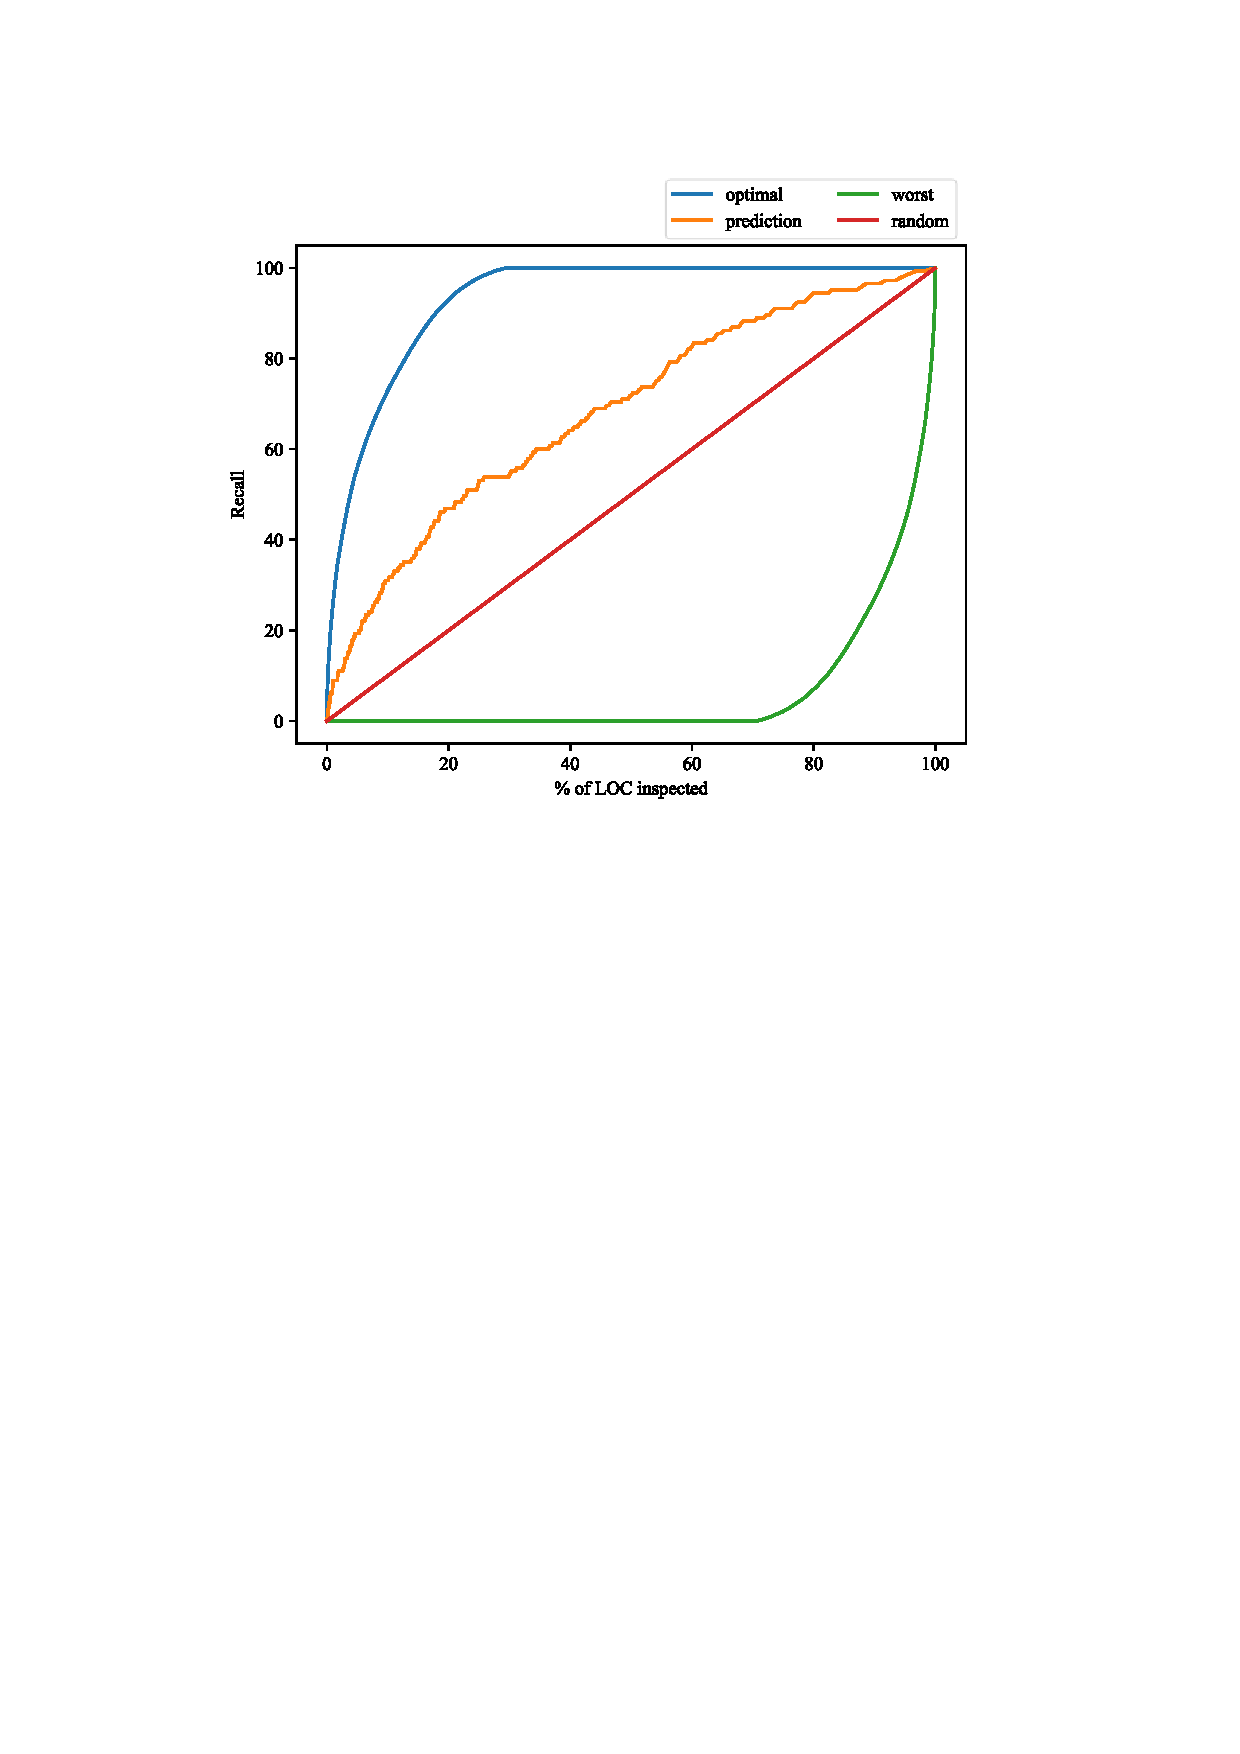
\includegraphics[scale=0.6]{figs/popt.pdf}
	\caption{An example of Alberg diagram}
	\label{fig_popt}
\end{figure}

\subsubsection{Win/Tie/Loss indicator}
%In order to better compare the performance of different models, we also apply the Win/Tie/Loss indicator, which is also used for performance comparison between different techniques by prior works~\cite{fan2019deep,liu2018connecting}. For each task, we repeat the model training and testing of our GH-LSTMs and other baseline models for 30 times. Then we conduct Wilcoxon signed-rank test and Cliff’s delta test to compare the performance of GH-LSTMs and other methods.

We also apply the Win/Tie/Loss indicator to compare the performance of different models further, which has been used in prior works for performance comparison between different methods~\cite{fan2019deep,liu2018connecting}. For each task, we repeat the model training and testing of our GH-LSTMs and other baseline models for 30 times. Then we conduct Wilcoxon signed-rank test and Cliff’s delta test to analyze the performance of GH-LSTMs and other methods.

The Wilcoxon signed-rank test is a non-parametric statistical hypothesis test used to determine whether two matched samples have the same distribution. If the $p$ value of Wilcoxon signed-rank test less than 0.05, then the difference between two matched samples is considered to be significantly different and otherwise not. To mitigate the effect caused by multiple tests, we conduct Benjamini-Hochberg correction~\cite{benjamini1995controlling} and report the BH-corrected $p$ values, which are used to calculate the Win/Tie/Loss indicator later.

%The Cliff's delta test is a non-parametric effect size measure that quantifies the amount of difference between two groups of observations beyond $p$ value interpretation. This measure can be understood as a useful complementary analysis for the corresponding hypothesis testing. Table~\ref{tab_delta} shows the mappings between the values of the Cliff's delta($|\delta|$) and their effective levels.
The Cliff's delta test is a non-parametric effect size test that measures the effective levels of difference between two sets of observation data, and can be regarded as a complementary analysis for the Wilcoxon signed-rank test. Table~\ref{tab_delta} shows the mappings between the Cliff's delta values($|\delta|$) and their effective levels.

\begin{table}[htbp]
	\footnotesize
	\caption{Mappings between the Cliff's delta values($|\delta|$) and their effective levels}
	\label{tab_delta}
	\tabcolsep 30pt
	\centering
	\begin{tabular}{ ll}
		\toprule
		Cliff's delta                  & Effective levels \\\midrule
		$|\delta| <$ 0.147             & Negligible       \\
		0.147 $\leq |\delta| <$ 0.33   & Small            \\
		0.33 $\leq |\delta| <$ 0.474   & Medium           \\
		0.474 $\leq |\delta|$         & Large             \\
		\bottomrule
	\end{tabular}
\end{table}

To be specific, we make the following comparisons to determine the result of Win/Tie/Loss indicator: for a baseline method M, if GH-LSTMs outperforms M with the $p$ value of Wilcoxon signed-rank test less than 0.05 and the Cliff's delta value greater than or equal to 0.147, the difference between these two models is statistical significant and can not be ignored. At this time, we mark the GH-LSTMs as a `Win'. In contrast, if the model M outperforms GH-LSTMs with a $p$ $<$0.05 and a Cliff's delta$\geq$0.147, GH-LSTMs will be marked as a `Loss'. Otherwise, we mark the case as a `Tie'. After all cases are marked, we calculate the Wins, Ties and Losses for GH-LSTMs against each technique on every task.



\subsection{Parameters setting}
Every defect prediction method implemented in this paper can be divided into two steps: feature extraction and classifier training. In the feature extraction phase, we set the same training parameters of GloVe model(used by SCE, DP-AM and GH-LSTMs) to generate the semantic features. To be specific, we set the embedding dimensions to be 40 and keep all other parameters as their default values\footnote{https://github.com/stanfordnlp/GloVe/blob/master/demo.sh}. As for the DBN model that generates DBN features, we stick to the original study~\cite{wang2018deep}, i.e., we set the number of hidden layers to 10, the number of nodes in each hidden layer to 100 and the number of iterations to 200. In the classifier training phase, we set the same parameters for all the LSTM networks used in GH-LSTMs and the baseline methods. Details of these parameters are shown in Table~\ref{tab_parameters}. Note that DP-AM uses a bidirectional RNN instead of LSTM and employs attention mechanism to boost performance, so we set the parameters of DP-AM according to the original study~\cite{fan2019deep}.

\begin{table*}[htbp]
	\footnotesize
	\caption{Hyper parameters for all LSTM networks}
	\label{tab_parameters}
	\tabcolsep 40pt
	\centering
	\begin{tabular}{ll}
		\toprule
		Parameter      & Description (value) \\\midrule
		LSTM units     & The number of the LSTM units in each layer (128). \\
		Batch size     & The number of training samples that are fed to LSTM at a time (2048). \\
		Epoch          & One forward/backward pass of all the training samples (200).         \\
		Optimizer      & The function that optimizes trainable parameters during training (adam).         \\
		Activation     & The activation function used in fully connected layers. (sigmoid).\\
		\bottomrule
	\end{tabular}
\end{table*}

\section{Experimental results}
In this section, we mainly focus on the following three research questions:

RQ1: How does GH-LSTMs perform under non-effort-aware scenario?

RQ2: How does GH-LSTMs perform under effort-aware scenario?

RQ3: How do external parameters affect the performance of GH-LSTMs?

The purpose of RQ1 and RQ2 is to verify the performance of GH-LSTM under the non-effort-aware scenario and the effort-aware scenario, respectively. RQ3 aims to explore how external parameters influence the performance of GH-LSTMs.

\subsection{Answer to RQ1: How does GH-LSTMs perform under non-effort-aware scenario?}

The results of $F-measure$ of all 16 sets of experiments are listed in the Table~\ref{tab_f}, and Fig.~\ref{fig_box_F-measure} shows the distribution of $F-measure$ values of 4 models on all tasks in the form of box-plot, from which we can have the observation that our GH-LSTMs outperforms all baseline methods in terms of median $F-measure$. In Table~\ref{tab_f}, the `Task' column stands for the project name and the corresponding versions used as training and testing sets. For example, `\textit{ant\_1.5\_1.6}' means this task uses the source files from version 1.5 of project \textit{ant} to build the training set that is used to train the defect prediction model, and uses source files from version 1.6 of project \textit{ant} to build the testing set to evaluate the performance of the trained model.


The `$F-measure$' column shows the $F-measure$ values of our proposed GH-LSTMs method and the other three baseline methods. For each task, the result of the best method is presented in bold. Generally speaking, on average, our GH-LSTMs model performs better than all the baseline models in terms of $F-measure$. Specifically, compared with DBN and SCE, our method makes an improvement in terms of $F-measure$ by 16.7 percentage points and 11.1 percentage points on average, which demonstrates the superiority of taking traditional features into consideration. On the other hand, our method outperforms DM-AP by 5.2 percentage points in terms of $F-measure$. Note that DM-AP leverages a more advanced bidirectional RNN based on attention mechanism and also makes use of traditional features by simply concatenating them and the extracted semantic information. This means that under non-effort-aware scenarios, our hierarchical architecture can extract more hidden information from traditional features, and our gated fusion strategy does a better job in feature combination than simple concatenation.


The `$p$($\delta$)' column shows $p$ values of Wilcoxon signed-rank test and Cliff's delta values. For the $p$ value of Wilcoxon signed-rank test, when the value is not less than 0.05, the original value is displayed; otherwise, it is replaced by `$<$0.05'. For Cliff's delta value, it is replaced by the effective level of Cliff's delta value. For the delta value of cliff, replace it with the effective level of cliff delta value. We add `+' or `-' before the effective level to discriminate the positive and negative Cliff's delta values. For example, compare GH-LSTMs with DBN on \textit{ant\_1.5\_1.6}, the $p$ value is less than 0.05 and the Cliff's delta value is 1.000($\geq$0.474), so the `$p$($\delta$)' of `GH-LSTMs vs. DBN' is `$<$0.05(+Large)', and according to the Win/Tie/Loss indicator, we can mark the GH-LSTMs as a `Win'. From the row `Average $\&$ Win/Tie/Loss' in Table~\ref{tab_f}, it can be seen that our GH-LSTMs model significantly outperforms other models in most tasks.



\begin{table*}[htbp]
	\scriptsize
	\caption{$F-measure$ values of DBN, SCE, DP-AM and GH-LSTMs}
	\label{tab_f}
	\tabcolsep 9pt
	\centering
	\begin{tabular}{m{2cm}|llll|lll}
		\toprule
		&\multicolumn{4}{c|}{$F-measure$}  &\multicolumn{3}{c}{$p$($\delta$)}   \\
		\midrule
		Task  &DBN  &SCE  &DP-AM  &GH-LSTMs  &GH-LSTMs vs. DBN  &GH-LSTMs vs. SCE  &GH-LSTMs vs. DP-AM   \\\midrule
		ant\_1.5\_1.6     &0.497     &0.284     &0.557     &\textbf{0.582}&$<$0.05(+Large)&$<$0.05(+Large)&$<$0.05(+Medium)\\
		ant\_1.6\_1.7     &0.305     &0.341     &0.522     &\textbf{0.584}&$<$0.05(+Large)&$<$0.05(+Large)&$<$0.05(+Large)\\
		camel\_1.2\_1.4   &0.228     &0.340     &0.393     &\textbf{0.415}&$<$0.05(+Large)&$<$0.05(+Large)&0.134(+Negligible)\\
		camel\_1.4\_1.6   &0.303     &0.398     &0.399     &\textbf{0.441}&$<$0.05(+Large)&0.075(+Small)&$<$0.05(+Medium)\\
		ivy\_1.4\_2.0     &0.086     &0.183     &0.321     &\textbf{0.393}&$<$0.05(+Large)&$<$0.05(+Large)&$<$0.05(+Large)\\
		jedit\_3.2\_4.0   &0.374     &0.465     &0.509     &\textbf{0.561}&$<$0.05(+Large)&$<$0.05(+Large)&$<$0.05(+Large)\\
		jedit\_4.0\_4.1   &0.421     &0.549     &0.553     &\textbf{0.634}&$<$0.05(+Large)&$<$0.05(+Large)&$<$0.05(+Large)\\
		log4j\_1.0\_1.1   &0.507     &0.621     &0.644     &\textbf{0.739}&$<$0.05(+Large)&$<$0.05(+Large)&$<$0.05(+Large)\\
		lucene\_2.0\_2.2  &\textbf{0.759}&0.710     &0.667     &0.734     &$<$0.05(-Large)&$<$0.05(+Medium)&$<$0.05(+Large)\\
		lucene\_2.2\_2.4  &0.482     &0.678     &0.707     &\textbf{0.743}&$<$0.05(+Large)&$<$0.05(+Large)&$<$0.05(+Medium)\\
		poi\_1.5\_2.5     &0.779     &0.829     &0.790     &\textbf{0.842}&$<$0.05(+Large)&$<$0.05(+Large)&$<$0.05(+Large)\\
		poi\_2.5\_3.0     &0.782     &0.776     &0.759     &\textbf{0.822}&$<$0.05(+Large)&$<$0.05(+Large)&$<$0.05(+Large)\\
		synapse\_1.0\_1.1 &0.349     &0.370     &0.440     &\textbf{0.464}&$<$0.05(+Large)&$<$0.05(+Large)&0.086(+Small)\\
		synapse\_1.1\_1.2 &0.299     &0.428     &0.517     &\textbf{0.605}&$<$0.05(+Large)&$<$0.05(+Large)&$<$0.05(+Large)\\
		xalan\_2.4\_2.5   &0.513     &0.584     &0.614     &\textbf{0.658}&$<$0.05(+Large)&$<$0.05(+Large)&$<$0.05(+Medium)\\
		xerces\_1.2\_1.3  &0.213     &0.239     &\textbf{0.347}&\textbf{0.347}&$<$0.05(+Large)&$<$0.05(+Large)&0.992(-Negligible)\\\midrule
		Average $\&$ Win/Tie/Loss&0.431&0.487&0.546&\textbf{0.598}&15/0/1&15/1/0&13/3/0\\
		\bottomrule
	\end{tabular}
\end{table*}

\begin{figure}[htbp]
	\centering
	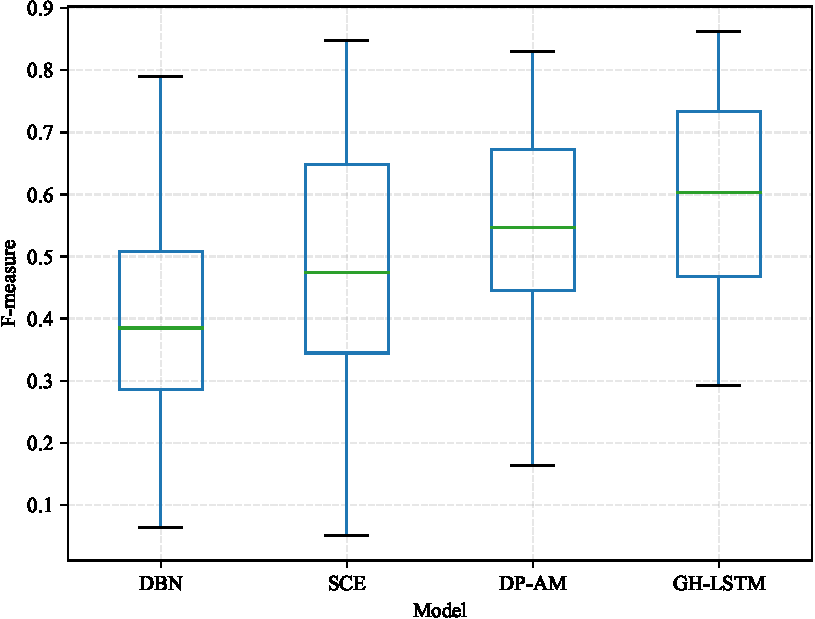
\includegraphics[scale=0.6]{figs/box_F-measure.pdf}
	\caption{Overall $F-measure$ comparison of DBN, SCE, DP-AM and GH-LSTMs}
	\label{fig_box_F-measure}
\end{figure}

In conclusion, the results of $F-measure$ show that: Feature fusion can effectively improve the performance of the model under non-effort-aware scenario: DP-AM and GH-LSTMs perform better than DBN and SCE, which is resulted from the ability of DP-AM and GH-LSTMs to combine both traditional features and semantic features; GH-LSTMs outperforms DP-AM(which combines two kinds of features by simple concatenation) because the hierarchical architecture is more effective in feature extraction and the gated fusion mechanism performs a better combination of two kinds of features.

\subsection{Answer to RQ2: How does GH-LSTMs perform under effort-aware scenario?}
To answer this question, we compare the performance of our proposed GH-LSTMs method with other baseline methods under effort-aware scenario using the $PofB20$, $IFA$ and $P_{opt}$. Table~\ref{tab_pof}, Table~\ref{tab_ifa} and Table~\ref{tab_popt} respectively show the performance of the four methods on $PofB20$, $IFA$ and $P_{opt}$.


Table~\ref{tab_pof} shows the $PofB20$ values of all 16 sets of experiments of our method and three baselines. For example, the $PofB20$ score of DBN on task `ant\_1.5\_1.6' is 0.261, which means by inspecting source code files in the decreasing order of defect probability given by the DBN method, we can detect 26.1\% real bugs when 20\% of the total lines of code are inspected. For each task, the highest $PofB20$ value is shown in bold. As we can see, GH-LSTMs outperforms other methods on most of the experiments(11 of 16). On average, our method outperforms DBN, SCE and DP-AM by 2.1 percentage points, 0.3 percentage points and 5.9 percentage points respectively. Additionally, according to the result of Win/Tie/Loss comparison, our GH-LSTMs model significantly outperforms SCE, i.e., the best baseline model, with 5 `Wins', 10 `Ties', and only 1 `Loss'. These results validate that GH-LSTMs method can detect more bugs under effort-aware scenarios. Moreover, the overall $PofB20$ comparison of 4 models is demonstrated in Fig.~\ref{fig_box_PofB20}, which shows that GH-LSTMs outperforms SCE in terms of minimum $PofB20$.


\begin{table*}[htbp]
	
	\scriptsize
	\caption{$PofB20$ scores of DBN, SCE, DP-AM and GH-LSTMs}
	\label{tab_pof}
	\tabcolsep 9pt
	\centering
	\begin{tabular}{m{2cm}|llll|lll}
		\toprule
		&\multicolumn{4}{c|}{PofB20}  &\multicolumn{3}{c}{$p$($\delta$)}   \\\midrule
		Task  &DBN  &SCE  &DP-AM  &GH-LSTMs  &GH-LSTMs vs. DBN  &GH-LSTMs vs. SCE  &GH-LSTMs vs. DP-AM\\\midrule
		ant\_1.5\_1.6     &\textbf{0.261}&0.249     &0.259     &0.260     &0.519(-Negligible)&$<$0.05(+Medium)&0.978(+Small)\\
		ant\_1.6\_1.7     &0.253     &0.279     &0.243     &\textbf{0.281}&$<$0.05(+Large)&0.172(+Small)&$<$0.05(+Large)\\
		camel\_1.2\_1.4   &\textbf{0.471}&0.469     &0.362     &0.469     &0.135(-Small)&0.779(+Negligible)&$<$0.05(+Large)\\
		camel\_1.4\_1.6   &0.508     &\textbf{0.559}&0.359     &0.555     &$<$0.05(+Large)&0.172(-Small)&$<$0.05(+Large)\\
		ivy\_1.4\_2.0     &0.161     &0.190     &\textbf{0.196}&\textbf{0.196}&$<$0.05(+Large)&$<$0.05(+Small)&0.580(+Negligible)\\
		jedit\_3.2\_4.0   &0.351     &0.390     &0.298     &\textbf{0.395}&$<$0.05(+Large)&0.511(+Negligible)&$<$0.05(+Large)\\
		jedit\_4.0\_4.1   &0.327     &0.362     &0.316     &\textbf{0.377}&$<$0.05(+Large)&$<$0.05(+Large)&$<$0.05(+Large)\\
		log4j\_1.0\_1.1   &0.265     &0.299     &0.275     &\textbf{0.320}&$<$0.05(+Large)&$<$0.05(+Medium)&$<$0.05(+Large)\\
		lucene\_2.0\_2.2  &\textbf{0.601}&0.593     &0.550     &0.594     &$<$0.05(-Large)&0.511(+Small)&$<$0.05(+Large)\\
		lucene\_2.2\_2.4  &\textbf{0.631}&0.619     &0.583     &0.618     &$<$0.05(-Large)&0.196(-Small)&$<$0.05(+Large)\\
		poi\_1.5\_2.5     &0.567     &\textbf{0.586}&0.524     &0.578     &$<$0.05(+Large)&$<$0.05(-Large)&$<$0.05(+Large)\\
		poi\_2.5\_3.0     &0.543     &0.546     &0.502     &\textbf{0.548}&$<$0.05(+Large)&$<$0.05(+Small)&$<$0.05(+Large)\\
		synapse\_1.0\_1.1 &0.267     &\textbf{0.289}&0.249     &0.279     &0.062(+Small)&0.172(-Small)&0.121(+Small)\\
		synapse\_1.1\_1.2 &0.298     &\textbf{0.313}&0.263     &0.311     &$<$0.05(+Large)&0.779(-Negligible)&$<$0.05(+Large)\\
		xalan\_2.4\_2.5   &0.598     &0.635     &0.532     &\textbf{0.636}&$<$0.05(+Large)&0.779(+Negligible)&$<$0.05(+Large)\\
		xerces\_1.2\_1.3  &0.657     &0.665     &0.637     &\textbf{0.668}&$<$0.05(+Large)&0.172(+Small)&0.251(+Negligible)\\\midrule
		Average $\&$ Win/Tie/Loss&0.422&0.440&0.384&\textbf{0.443}&11/3/2&5/10/1&12/4/0\\
		\bottomrule
	\end{tabular}
\end{table*}

\begin{figure*}
\centering
\begin{minipage}[b]{.45\textwidth}
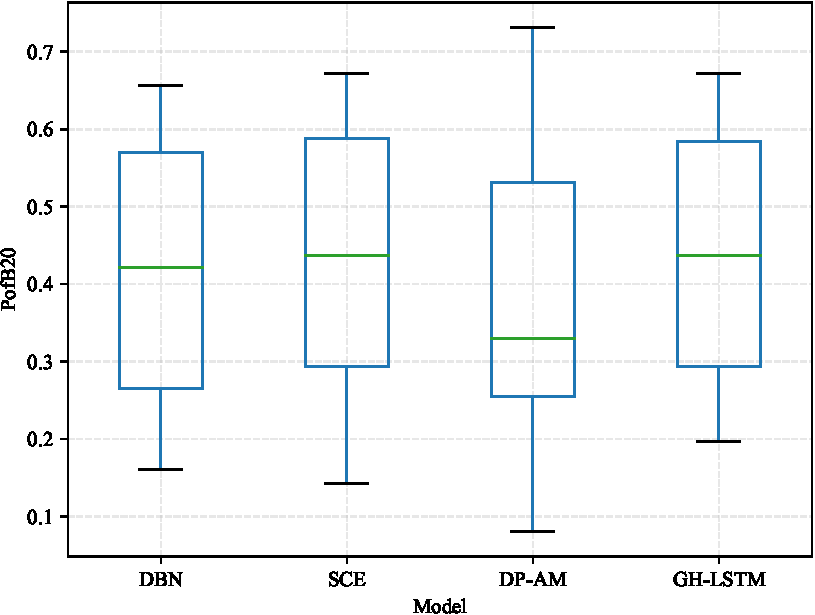
\includegraphics[scale=0.6]{figs/box_PofB20.pdf}
\caption{Overall $PofB20$ comparison of DBN, SCE, DP-AM and GH-LSTMs}
\label{fig_box_PofB20}
\end{minipage}\qquad
\begin{minipage}[b]{.45\textwidth}
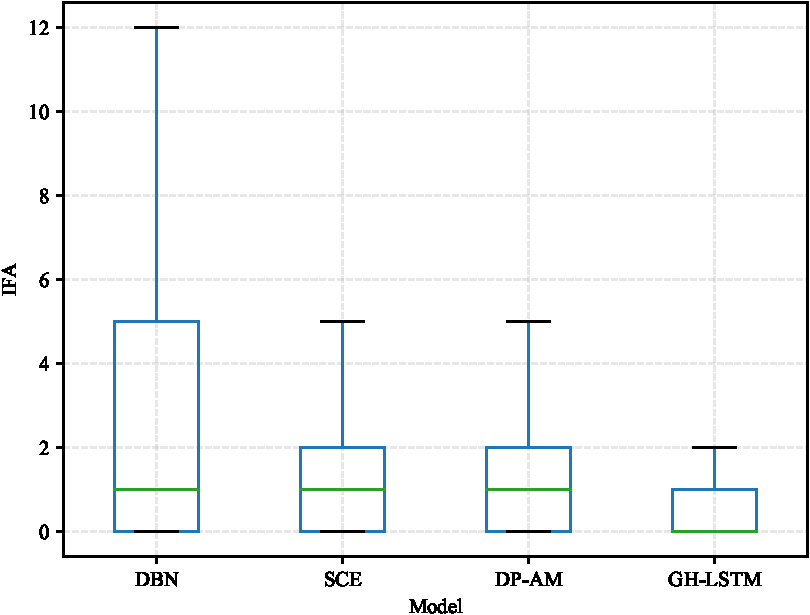
\includegraphics[scale=0.6]{figs/box_IFA.pdf}
		\caption{Overall $IFA$ comparison of DBN, SCE, DP-AM and GH-LSTMs}
		\label{fig_box_IFA}
\end{minipage}
\end{figure*}




From Table~\ref{tab_ifa}, we can have the following observations: Firstly, on average, our GH-LSTMs model significantly outperforms the other three models in terms of $IFA$ with the average value of 0.617, while the $IFA$ values of other three models are 5.004, 1.667 and 4.546. Secondly, SCE and GH-LSTMs perform much better than the other two baselines, and SCE is actually a part of GH-LSTMs, i.e., the semantic-level LSTM without the gated fusion mechanism. This indicates that LSTM is a better learning algorithm to further extract the semantic information from word embeddings under effort-aware scenarios. This conclusion is also supported by the results shown in Fig.~\ref{fig_box_IFA}, where the overall distribution of $IFA$ of all 4 methods is presented. Note that the lower the $IFA$ value is, the better the model performs. Therefore, as indicated in Fig.~\ref{fig_box_IFA}, our GH-LSTMs significantly outperforms all baseline methods in terms of $IFA$.

\begin{table*}[t]
	\scriptsize
	\caption{$IFA$ of DBN, SCE, DP-AM and GH-LSTMs}
	\label{tab_ifa}
	\tabcolsep 9pt
	\centering
	\begin{tabular}{m{2cm}|llll|lll}
		\toprule
		&\multicolumn{4}{c|}{IFA}  &\multicolumn{3}{c}{$p$($\delta$)}   \\\midrule
		Task  &DBN  &SCE  &DP-AM  &GH-LSTMs  &GH-LSTMs vs. DBN  &GH-LSTMs vs. SCE  &GH-LSTMs vs. DP-AM   \\\midrule
		ant\_1.5\_1.6     &2.100     &3.133     &4.900     &\textbf{1.133}&$<$0.05(-Medium)&0.066(-Small)&0.706(+Small)\\
		ant\_1.6\_1.7     &5.433     &2.567     &16.100    &\textbf{0.500}&$<$0.05(-Large)&$<$0.05(-Small)&0.092(-Negligible)\\
		camel\_1.2\_1.4   &18.967    &1.067     &3.900     &\textbf{0.000}&$<$0.05(-Large)&$<$0.05(-Medium)&$<$0.05(-Medium)\\
		camel\_1.4\_1.6   &2.500     &2.300     &4.300     &\textbf{1.767}&0.174(-Small)&0.315(-Small)&0.550(-Negligible)\\
		ivy\_1.4\_2.0     &27.567    &2.767     &13.100    &\textbf{0.567}&$<$0.05(-Large)&$<$0.05(-Large)&$<$0.05(-Small)\\
		jedit\_3.2\_4.0   &1.567     &0.733     &5.533     &\textbf{0.133}&$<$0.05(-Large)&$<$0.05(-Medium)&$<$0.05(-Large)\\
		jedit\_4.0\_4.1   &1.900     &2.667     &6.900     &\textbf{0.400}&0.067(-Small)&$<$0.05(-Large)&$<$0.05(-Large)\\
		log4j\_1.0\_1.1   &6.367     &0.767     &1.467     &\textbf{0.033}&$<$0.05(-Large)&$<$0.05(-Large)&$<$0.05(-Medium)\\
		lucene\_2.0\_2.2  &1.000     &0.767     &0.400     &\textbf{0.333}&$<$0.05(-Large)&0.121(-Small)&0.914(+Negligible)\\
		lucene\_2.2\_2.4  &\textbf{0.100}&0.200     &0.933     &0.200     &0.562(+Negligible)&0.785(-Negligible)&$<$0.05(-Medium)\\
		poi\_1.5\_2.5     &0.167     &\textbf{0.100}&2.133     &0.133     &0.854(-Negligible)&0.785(+Negligible)&0.095(-Small)\\
		poi\_2.5\_3.0     &0.767     &0.100     &0.367     &\textbf{0.000}&$<$0.05(-Small)&0.121(-Negligible)&$<$0.05(-Small)\\
		synapse\_1.0\_1.1 &2.633     &2.433     &1.567     &\textbf{0.433}&$<$0.05(-Large)&$<$0.05(-Large)&$<$0.05(-Medium)\\
		synapse\_1.1\_1.2 &\textbf{0.733}&2.100     &4.333     &1.367     &$<$0.05(+Large)&0.213(-Negligible)&0.111(-Negligible)\\
		xalan\_2.4\_2.5   &1.567     &0.467     &\textbf{0.433}&0.733     &$<$0.05(-Medium)&0.735(+Negligible)&0.425(+Negligible)\\
		xerces\_1.2\_1.3  &6.700     &4.500     &6.367     &\textbf{2.133}&$<$0.05(-Medium)&$<$0.05(-Medium)&$<$0.05(-Small)\\\midrule
		Average $\&$ Win/Tie/Loss&5.004&1.667&4.546&\textbf{0.617}&11/4/1&8/8/0&9/7/0\\
		\bottomrule
	\end{tabular}
\end{table*}


Table~\ref{tab_popt} shows $P_{opt}$ scores of four models. We can see that GH-LSTMs significantly outperforms DBN and DP-AM according to the results of Win/Tie/Loss. Besides, although the SCE model is slightly better than the other three models in terms of average value, from the Win/Tie/Loss results, our GH-LSTMs model has 5 `Wins' and only 2 `Losses' in comparison to SCE, which means that GH-LSTMs significantly outperforms SCE on more tasks. Fig.~\ref{fig_box_Popt} shows the distribution of $P_{opt}$ scores of DBN, SCE, DP-AM and GH-LSTMs on all tasks, from which we can also see that GH-LSTMs achieves comparable performance with SCE.

\begin{table*}[t]
	\scriptsize
	\caption{$P_{opt}$ scores of DBN, SCE, DP-AM and GH-LSTMs}
	\label{tab_popt}
	\tabcolsep 9pt
	\centering
	\begin{tabular}{m{2cm}|llll|lll}
		\toprule
		&\multicolumn{4}{c|}{$P_{opt}$}  &\multicolumn{3}{c}{$p$($\delta$)}   \\\midrule
		Task  &DBN  &SCE  &DP-AM  &GH-LSTMs  &GH-LSTMs vs. DBN  &GH-LSTMs vs. SCE  &GH-LSTMs vs. DP-AM   \\\midrule
		ant\_1.5\_1.6     &\textbf{0.654}&0.642     &0.616     &0.651     &$<$0.05(-Large)&$<$0.05(+Large)&$<$0.05(+Large)\\
		ant\_1.6\_1.7     &0.610     &\textbf{0.611}&0.574     &\textbf{0.611}&$<$0.05(+Medium)&0.105(-Small)&$<$0.05(+Large)\\
		camel\_1.2\_1.4   &0.708     &\textbf{0.724}&0.630     &0.721     &$<$0.05(+Large)&0.060(-Medium)&$<$0.05(+Large)\\
		camel\_1.4\_1.6   &0.755     &\textbf{0.775}&0.593     &0.774     &$<$0.05(+Large)&0.926(-Negligible)&$<$0.05(+Large)\\
		ivy\_1.4\_2.0     &0.574     &0.595     &0.565     &\textbf{0.596}&$<$0.05(+Large)&0.557(+Negligible)&$<$0.05(+Large)\\
		jedit\_3.2\_4.0   &0.734     &\textbf{0.748}&0.653     &0.747     &$<$0.05(+Large)&0.495(-Small)&$<$0.05(+Large)\\
		jedit\_4.0\_4.1   &0.699     &\textbf{0.722}&0.635     &0.719     &$<$0.05(+Large)&0.279(-Small)&$<$0.05(+Large)\\
		log4j\_1.0\_1.1   &0.619     &\textbf{0.665}&0.592     &0.663     &$<$0.05(+Large)&0.591(-Negligible)&$<$0.05(+Large)\\
		lucene\_2.0\_2.2  &0.895     &0.895     &0.837     &\textbf{0.896}&$<$0.05(+Large)&$<$0.05(+Medium)&$<$0.05(+Large)\\
		lucene\_2.2\_2.4  &\textbf{0.909}&0.903     &0.863     &0.906     &$<$0.05(-Large)&$<$0.05(+Large)&$<$0.05(+Large)\\
		poi\_1.5\_2.5     &0.904     &\textbf{0.916}&0.849     &0.909     &$<$0.05(+Large)&$<$0.05(-Large)&$<$0.05(+Large)\\
		poi\_2.5\_3.0     &0.902     &\textbf{0.904}&0.849     &\textbf{0.904}&$<$0.05(+Large)&0.105(+Small)&$<$0.05(+Large)\\
		synapse\_1.0\_1.1 &0.721     &\textbf{0.733}&0.597     &0.724     &$<$0.05(+Large)&$<$0.05(-Large)&$<$0.05(+Medium)\\
		synapse\_1.1\_1.2 &0.717     &0.741     &0.651     &\textbf{0.742}&$<$0.05(+Large)&0.926(-Negligible)&$<$0.05(+Large)\\
		xalan\_2.4\_2.5   &0.869     &0.890     &0.786     &\textbf{0.891}&$<$0.05(+Large)&$<$0.05(+Small)&$<$0.05(+Large)\\
		xerces\_1.2\_1.3  &0.843     &0.847     &0.796     &\textbf{0.848}&$<$0.05(+Large)&$<$0.05(+Medium)&$<$0.05(+Large)\\\midrule
		Average $\&$ Win/Tie/Loss&0.757&\textbf{0.770}&0.693&0.769&14/0/2&5/9/2&16/0/0\\
		\bottomrule
	\end{tabular}
\end{table*}

\begin{figure}[htbp]
	\centering
	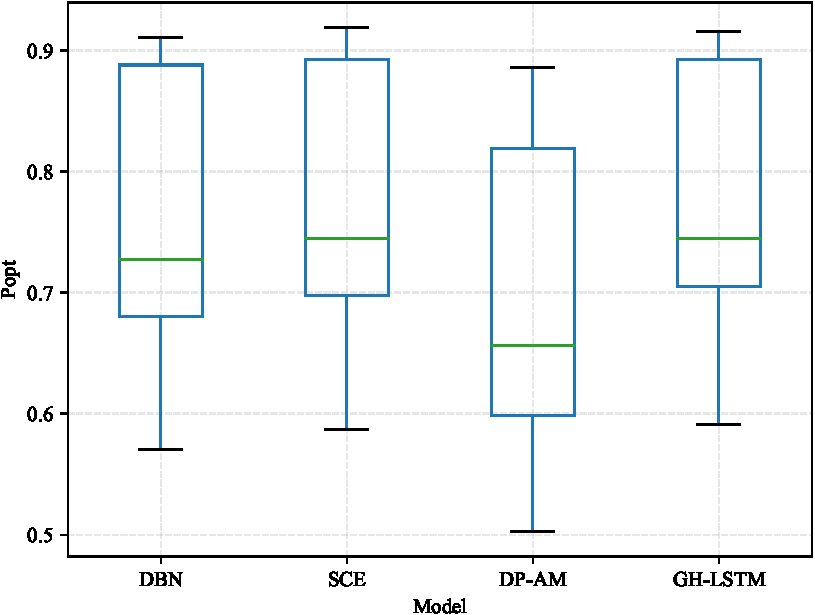
\includegraphics[scale=0.6]{figs/box_Popt.pdf}
	\caption{Overall $P_{opt}$ comparison of DBN, SCE, DP-AM and GH-LSTMs}
	\label{fig_box_Popt}
\end{figure}

In conclusion, GH-LSTMs significantly outperformed the other three baselines when evaluated by $PofB20$ and $IFA$, and achieved comparable performance with SCE when evaluated by $P_{opt}$. These results indicate that benefiting from hierarchical architecture and proper gated feature fusion mechanism, GH-LSTMs is able to give more accurate prediction results under effort-aware scenario.

\subsection{Answer to RQ3: How do external parameters affect the performance of GH-LSTMs?}
In this part, we will make a discussion about two external parameters that may affect the performance of GH-LSTMs model: dimensions of semantic code embedding and the size of training set.

To figure out how the dimensions of semantic code embedding influences the prediction performance of GH-LSTMs, we retrain the GloVe models with 5 different dimension parameters of 10d, 20d, 30d, 40d(original), 50d and regenerate semantic features using corresponding GloVe model. On the other hand, the traditional features remain the same as the original experiments. The $F-measure$ values of these 16 tasks with 5 different dimensions are listed in Fig.~\ref{fig_dimensions}.

As Fig.~\ref{fig_dimensions} shows, the dimensions of the semantic code embedding have no significant impact on classification performance: The average performance fluctuation of all 16 tasks is 0.024 in terms of $F-measure$ and the greatest performance fluctuation appears in task `came\_1.4\_1.6', where increasing dimensions boost the $F-measure$ by 0.048. Considering that the datasets used to build semantic corpus in our experiments are much smaller than those in common NLP tasks, we can draw a conclusion that semantic code embedding with lower dimensions would not cause obvious performance variation for our GH-LSTM method on datasets with similar scale. Therefore, our advice is: if you use the datasets that have similar scale to our datesets, a fine-tuning of dimensions of semantic code embedding will be helpful to find the lowest usable dimension, which will leads to less consumption in training and testing process with equal levels of performance.

\begin{figure}[h]
	\centering
	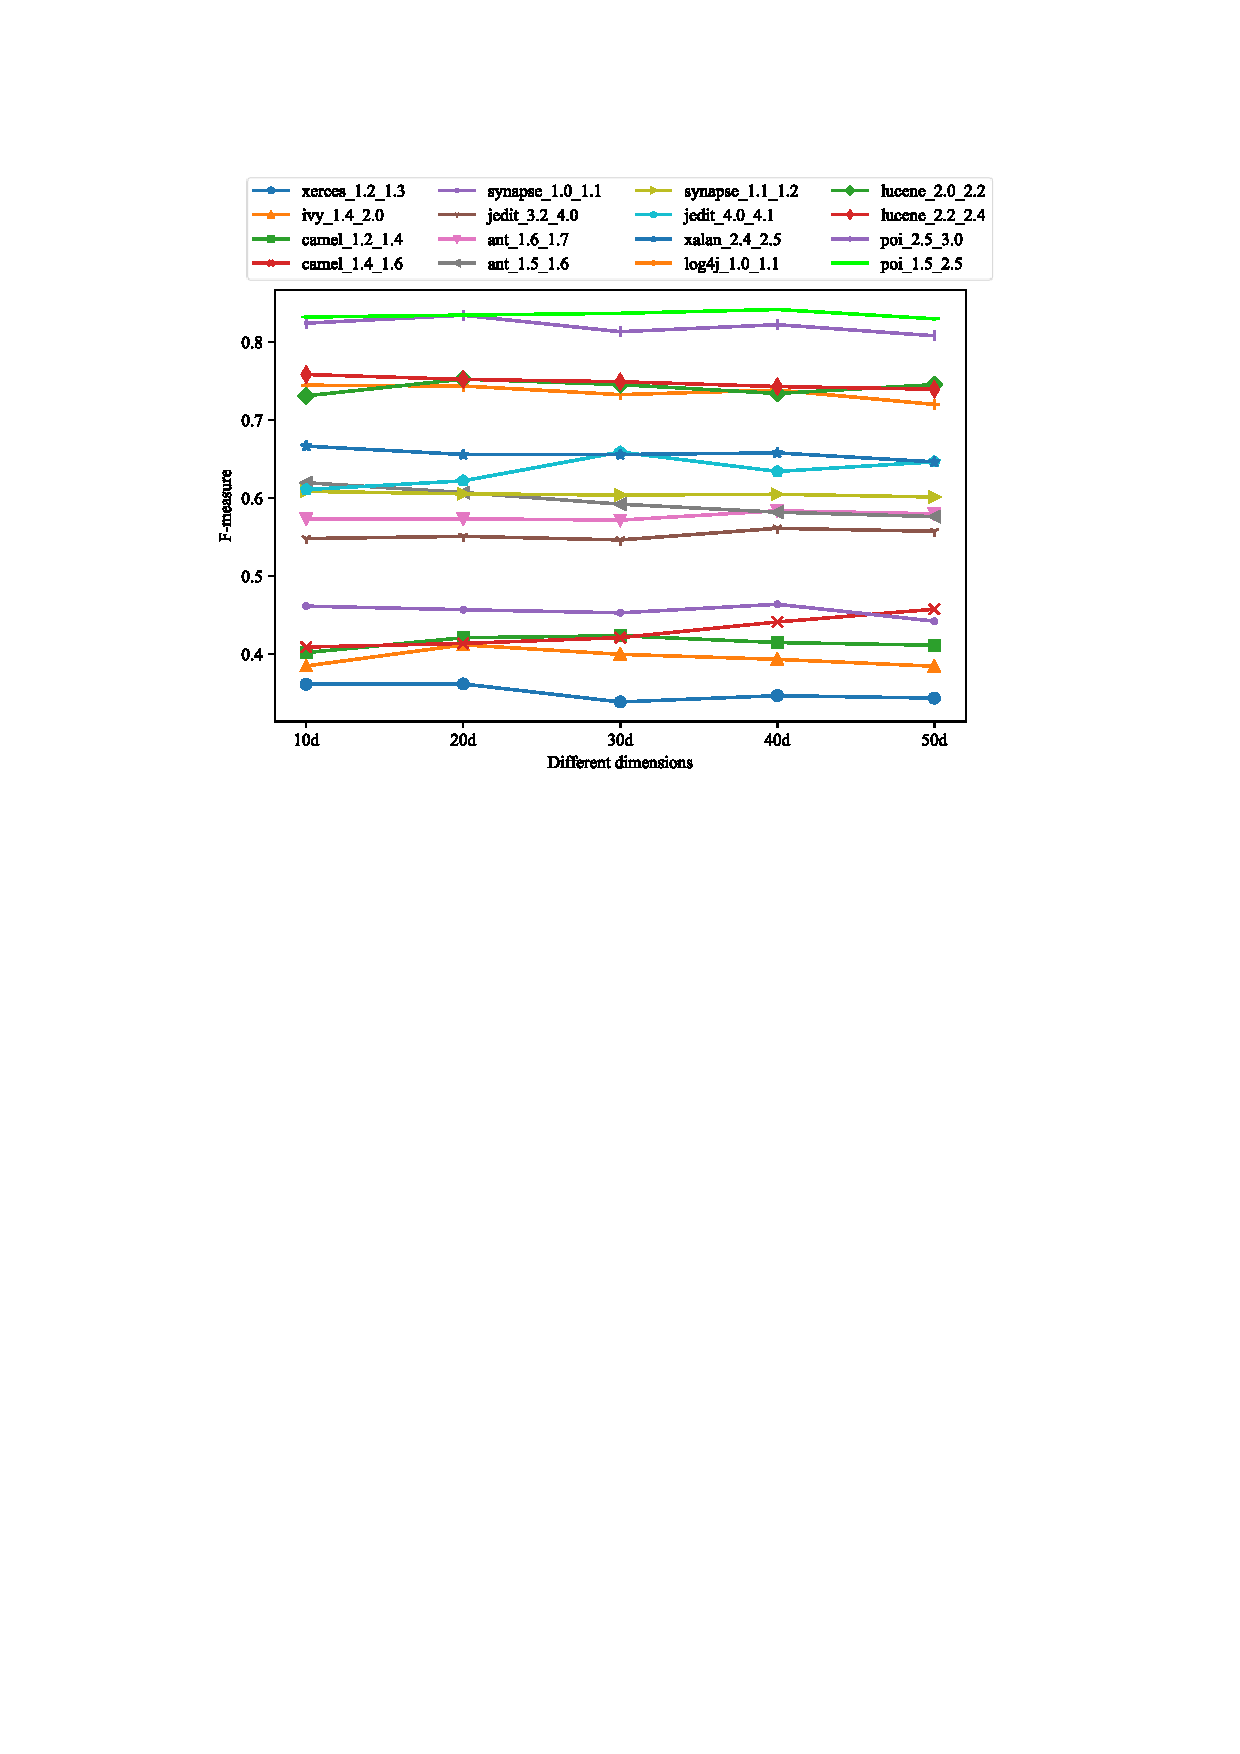
\includegraphics[scale=0.6]{figs/dimensions.pdf}
	\caption{F-measure of GH-LSTMs under different embedding dimensions}
	\label{fig_dimensions}
\end{figure}

Since GH-LSTMs is a deep learning model, the size of the training set, i.e., the scale of the training version of the project, is possible to have effects on the learning process of the model. Since the defect distribution is usually project-specific, it is inappropriate to compare the performance of all the tasks directly. In order to estimate the performance of GH-LSTMs under different sizes of training sets, we built new training sets that are obtained by under-sampling from the original training sets. We choose under-sampling rather than over-sampling because the new training sets generated by under-sampling only consist of real instances, which is more suitable under the setting of this discussion. Specifically, we select 3 sets of experiments that have the largest sizes of training sets and then perform an under-sampling operation on these training sets. We ensure the defect rate remains the same as the original training sets and set the new sizes of training sets to 25\%, 50\%, 75\% and 100\% of the original training sets. Fig.~\ref{fig_size} shows the performance of GH-LSTMs with different sizes of training sets.

\begin{figure}[h]
	\centering
	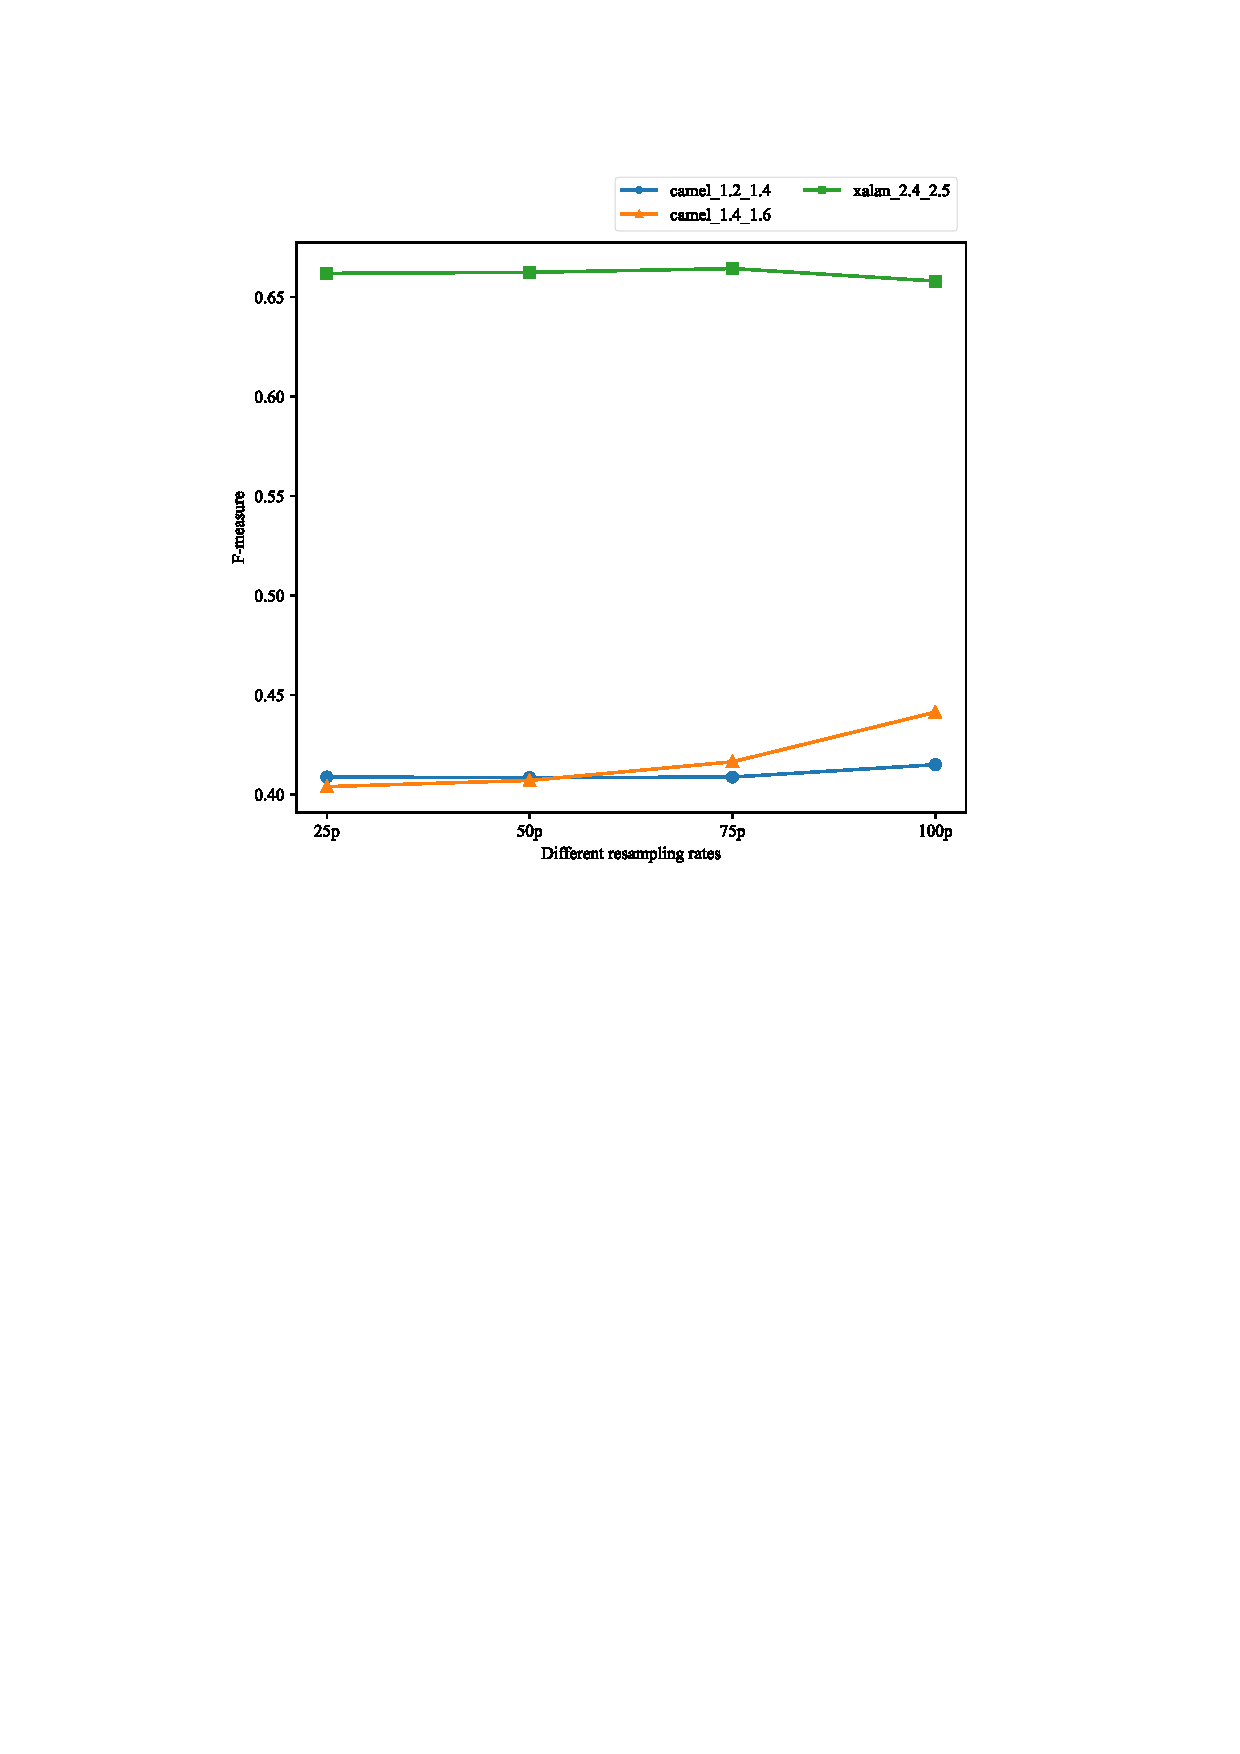
\includegraphics[scale=0.6]{figs/resampling_rates.pdf}
	\caption{F-measure of GH-LSTMs under different sizes of training sets}
	\label{fig_size}
\end{figure}
From Fig.~\ref{fig_size}, we can have the following observation: generally speaking, the GH-LSTMs models trained on under-sampled training sets achieve similar performance when compared with the original GH-LSTMs models. The performance fluctuations caused by changed sizes of training sets are less than 1 percentage points in most cases in terms of $F-measure$(with only one exception for task `came\_1.4\_1.6' where the size of training set changing from `75\% - 100\%' results in 2.8 percentage points of performance variation). Since we adopt this under-sampling strategy, these results can be considered as the approximation of the real applications. Therefore, we can draw a conclusion that the performance of GH-LSTMs is not likely to be seriously influenced by the size of the training set when the defect distribution remains unchanged.


\section{Threats to validity}
\subsection{Internal validity}
%Internal validity is the degree of confidence that the causal relationship being tested is trustworthy and not influenced by other factors or variables. The major threat to internal validity is the correctness of our experiment environment. First, we used Keras to build the GH-LSTMs model that we used in our research. The backend of Keras we used is Tensorflow. For the word vectors initialization, we used Glove to initialize the vectors. These tools mentioned above are widely used in related works and considered to be reliable. Furthermore, to ensure that the models used in our experiments are correctly implemented, we have conducted white-box testing on source code such as peer code review and logic coverage-based test case execution.

Internal validity refers to the degree of confidence to which the causal relationship studied in a research is independent of other factors, i.e., is not affected by other variables. Therefore, the correctness of our experimental environment is significant for internal validity. In this study, we build the GH-LSTMs model by Keras and use Tensorflow as the backend of Keras. Additionally, we utilize GloVe to initialize the word vectors. These tools and technologies should be considered reliable since they have been widely used in related researches. Finally, to ensure that the code used to build the model in our experiments is error-free, we also conduct white-box testing on the source code.
\subsection{External validity}
%External validity is the extent to which results form a study can be generalized to other situations. The main threat to external validity is that we only use 10 Java projects in PROMISE. They do not represent all projects (such as other Java projects and non-Java projects). Further validation on various datasets is desirable to help generalize our findings. What is more, the runtime of our model may vary depending on the hardware configuration.
External validity refers to the validity of a scientific research result that can be applied to other studies. The main threat to external validity in this study is that we only use 10 Java projects in PROMISE repository. They do not represent all projects (such as other Java projects and non-Java projects). Experiments on other datasets will help to further verify the validity of our method.
\subsection{Construct validity}
Construct validity refers to the degree to which the independent variables and dependent variables really represent the concepts that we are interested in measuring. The independent variables in our study can be divided into semantic features and traditional features. The semantic features are extracted from ASTs of source code files using word embedding technique, which is proved effective by previous studies~\cite{liang2019seml,fan2019deep}. Additionally, we select 18 code metrics provided by the PROMISE repository as traditional features. These code metrics are calculated by the CKJM tool~\cite{jureczko2010towards}. For dependent variables, we use bug label data that identified by the BugInfo tool~\cite{jureczko2010using} from the PROMISE repository, based on which a lot of studies has been conducted ~\cite{wang2018deep,liang2019seml,fan2019deep}. To sum up, the construct validity of the independent variables and dependent variables of this paper should be acceptable.

%As for the construct validity, the main threat involves the measurement. We choose 4 widely-used metrics on the testing dataset to measure and compare the performance of models. We choose the datasets in PROMISE repository, and a lot of research is based on these datasets. Therefore, the quality of the test datasets should be acceptable.
\subsection{Conclusion validity}
%Conclusion validity is the degree to which conclusions we reach about relationships in our data are reasonable. There is little threat to conclusion validity in our study. To mitigate it, a large number of experimental trials have been conducted for each model, as well as each dataset. These trials have resulted in sufficiently huge experimental data, which helped us obtain statistically reliable results.
Conclusion validity refers to the extent to which the research conclusion is drawn in a reasonable way. In this study, to mitigate the threat to conclusion validity, we carry out a large number of experiments on enough projects for each model, thus the results obtained from the generated experimental data should be statistically reliable. 

\section{Related works}
\subsection{Traditional software defect prediction}
%Most defect prediction techniques focus on manually designing new discriminative features or new combinations of features from labeled historical defect data, which are fed into machine learning based classifiers to identify software defects. These features can be categorized as static features and process features.
Software defect prediction is a research hotspot in the field of software engineering, around which a lot of work has been carried out~\cite{wang2018deep,fan2019deep,menzies2006data}. 
Most defect prediction techniques are focused on proposing new discriminative features that can be generated from the history information of software. These features, including static features and process features, will be fed into classifiers to identify software defects. Static features such as LOC are based on the static information of software modules, i.e., the source code files, while process features are usually extracted by analyzing changes of software modules such as code delta feature~\cite{nagappan2010change} and code turn feature~\cite{nagappan2005use}.


Among the existing software defect prediction studies, traditional machine learning methods are commonly used~\cite{elish2008predicting,wen2012systematic}. Catalyst and Diri~\cite{catal2009investigating} selected Random Forest, C4.5, Naive Bayes and other machine learning algorithms to conduct experiments. The experimental results show that the performance of the Random Forest is the best on the large-scale datasets, while the performance of Naive Bayes is the best on the small-scale datasets. When the feature selection technique is used, the performance of the Random Forest model remains the best. Elish et al.~\cite{elish2008predicting} compared the performance of eight modeling techniques with Support Vector Machine(SVM) using NASA datasets. As the experimental results show, the SVM method generally achieves better performance than other comparable models. In cross-project software defect prediction, Ryu et al.~\cite{ryu2016value} proposed a SVM boosting method, which applied imbalance processing technology in the cross-project defect prediction, and the experimental results prove that their method can achieve better performance.

%The experimental results indicate that the prediction performance of SVM is generally better than, or at least, is competitive against the compared models.

\subsection{Deep learning in software defect prediction}
In recent years, with the popularity of artificial neural networks, researchers have begun to apply deep learning techniques to the field of software defect prediction. Yang et al.~\cite{yang2015deep} used DBN to generate expressive features from a set of initial change features in just-in-time defect prediction. Compared with the method proposed by previous work~\cite{kamei2007effects}, their method performs better in terms of 4 metrics on 6 open-source projects. Liu et al.~\cite{liu2018connecting} proposed to utilize the Historical Version Sequence of Metrics (HVSM), which can be extracted from continuous versions software, to build software prediction models based on RNN. Wang et al.~\cite{wang2018deep} designed the semantic feature by using DBN to extract semantic information from token vectors generated from AST node sequences and achieved better performance in both with-in project and cross-project software defect prediction. Liang et al.~\cite{liang2019seml} proposed another semantic feature represented in the form of word embedding and chose LSTM as the classifier to boost the performance of defect prediction. To make use of the combination of semantic features and traditional features, Fan et al.~\cite{fan2019deep} proposed a framework called DP-AM, which leverages a bidirectional RNN with attention mechanism and combines traditional features with semantic features for better performance. Different from their method where traditional features are appended to semantic features by simple concatenation, our GH-LSTMs model leverages a hierarchical architecture to extract both kinds of features efficiently and adopts the gated feature fusion layer to properly combine the extracted features.


Hierarchical network architectures are widely used in typical deep learning areas such as natural language processing and computer vision. For example, in order to make full use of both intra-sentence and inter-sentence relations, Ruder et al. proposed a hierarchical model, which stacks a review-level Bi-LSTM on top of the sentence-level Bi-LSTM. In this paper, we introduce a gated hierarchical LSTMs network to perform defect prediction. To the best of our knowledge, this is the first time that hierarchical architecture is used to perform defect prediction tasks.

%Ruder et al.~\cite{ruder2016hierarchical} yielded a hierarchical LSTMs method by stacking a review-level Bi-LSTM on the top of a sentence-level Bi-LSTM, which is able to leverage both intra-sentence and inter-sentence relations. This model inspires us to use a gated hierarchical LSTMs model to utilize both traditional features and semantic features.

\section{Conclusion and future work}
With the increasing complexity and scale of software products, reliability assurance has become a significant challenge. In this paper, we propose a deep-learning-based method called GH-LSTMs, which predicting potential code defects in software modules. GH-LSTMs can further extract semantic features and traditional features simultaneously using the hierarchical LSTMs architecture, and then we utilize gated merge mechanism to automatically learn the optimal ratio of feature fusion to make the best use of both semantic features and traditional features. Finally, the combined features are fed to a fully-connected layer to perform the task of with-in project defect prediction. We conducted 16 sets of experiments on 10 open source projects. The results indicate that our proposed GH-LSTMs method significantly outperforms the state-of-the-art method in terms of $F-measure$ under non-effort-aware scenario. Moreover, under effort-aware scenario, when compared with the state-of-the-art methods, GH-LSTMs significantly outperforms them in terms of $PofB20$ and $IFA$, and achieves comparable performance in terms of $P_{opt}$.

As for future work, we would like to further explore the performance of GH-LSTMs in cross-project defect prediction tasks. Additionally, it is of great value to extend our method to other programming languages such as C and C++.



\section*{Acknowledgements}

This work is partially supported by National Natural Science Foundation of China(61772263, 61772014), Collaborative Innovation Center of Novel Software Technology and Industrialization, Suzhou Technology Development Plan(key industry technology innovation-prospective application research project SYG201807), and the Priority Academic Program Development of Jiangsu Higher Education Institutions.


%% Loading bibliography style file
%\bibliographystyle{model1-num-names}
\bibliographystyle{IEEEtran}

% Loading bibliography database
\bibliography{IEEEtran}

\clearpage

\begin{IEEEbiography}[{
\includegraphics[width=2.8cm,height=3.5cm,clip,keepaspectratio]{./IEEEbiography/Hao_Wang.pdf}}]{Hao Wang}
is now a Master degree candidate in the School of Computer Science and Technology, Soochow University, China. He received his B.E. degree at Soochow University. 

His research interests include software defect prediction and natural language processing.
\end{IEEEbiography}


\begin{IEEEbiography}[{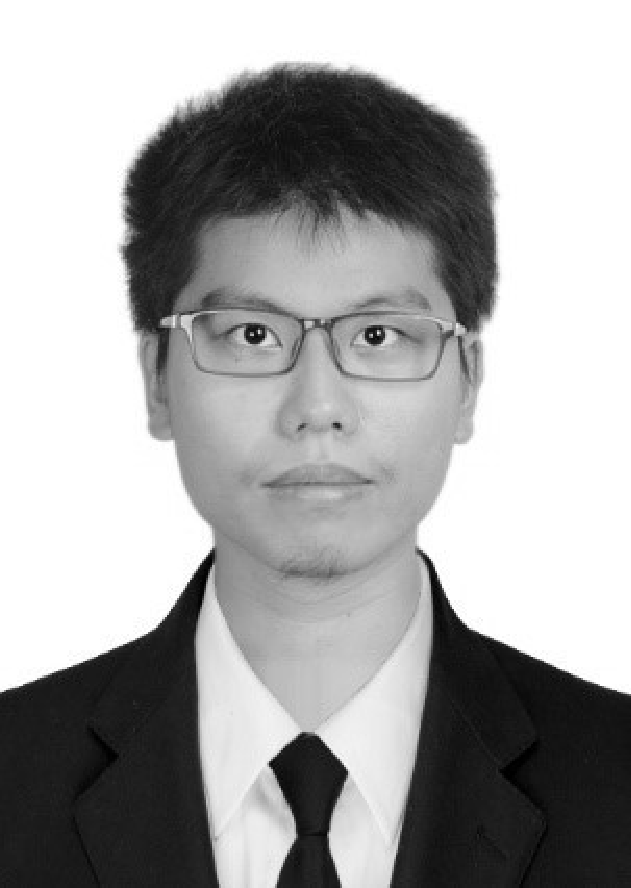
\includegraphics[width=2.8cm,height=3.5cm,clip,keepaspectratio]{./IEEEbiography/Weiyuan_Zhuang.pdf}}]{Weiyuan Zhuang}
is now a Master degree candidate in the School of Computer Science and Technology, Soochow University, China. He received his B.E. degree at Soochow University. 

His research interests include software defect prediction and deep learning.
\end{IEEEbiography}


\begin{IEEEbiography}[{
\includegraphics[width=2.8cm,height=3.5cm,clip,keepaspectratio]{./IEEEbiography/Xiaofang_Zhang.pdf}}]{Xiaofang Zhang}
is an Associate Professor in the School of Computer Science and Technology, Soochow University, China. 

Her research interests lie primarily in the intersection of Software Engineering and Artificial Intelligence, including intelligent software engineering, software testing, and software defect prediction.
\end{IEEEbiography}

\end{document}

